\documentclass[twoside]{book}
%=========== PACKAGES ============================
\usepackage{amsmath,amsthm,amssymb,physics,amsfonts}          %math packages
\usepackage[a4paper, total={6in, 8in}, margin=2cm]{geometry}     %margine
\usepackage{xcolor}         % Extended colors
\usepackage{color}         % Color extended names
\usepackage[many]{tcolorbox}
\usepackage{mwe}         % titlepage
\usepackage[bitstream-charter]{mathdesign}
\usepackage[colorlinks=true,linkcolor=blue]{hyperref}  %hyperlinking def,thm,..
\usepackage[frak=esstix]{mathalpha}
\usepackage[style=authoryear]{biblatex}
\usepackage{mathtools,leftindex,tensor,mhchem}
\usepackage{enumitem}
\usepackage{bbding}
\usepackage{tikz}
\usepackage{mathrsfs,relsize,array}
\newcommand\Laplace{\mathlarger{\mathlarger{\mathscr{L}}}}
\usepackage{setspace}
\spacing{1.2}
\usepackage{subfig}
\usepackage{emptypage}

%============Define colors ===========================
\definecolor{problemblue}{RGB}{100,134,158}    % for Exercise
\definecolor{idiomsgreen}{RGB}{0,162,0}         % for Exercise
\definecolor{exercisebgblue}{RGB}{192,232,252}      % for Exercise
\definecolor{myblue}{RGB}{0,163,243}  % for theorem
%\definecolor{myblue}{RGB}{242,1,11}  % for theorem
%\definecolor{myblue}{RGB}{241,199,16}  % for theorem
\definecolor{myOrange}{RGB}{255,178,102}  % for proposition

%============Laplace ==================================
\usepackage{mathrsfs}
\newsavebox\foobox
\newlength{\foodim}
\newcommand{\slantbox}[2][0]{\mbox{%
        \sbox{\foobox}{#2}%
        \foodim=#1\wd\foobox
        \hskip \wd\foobox
        \hskip -0.5\foodim
        \pdfsave
        \pdfsetmatrix{1 0 #1 1}%
        \llap{\usebox{\foobox}}%
        \pdfrestore
        \hskip 0.5\foodim
    }}
\def\Laplace{\slantbox[-.45]{$\mathscr{L}$}}
%================ derivatives ============================
\usepackage[mathscr]{euscript}

% Copied from mathrsfs.sty
\DeclareSymbolFont{rsfs}{U}{rsfs}{m}{n}
\DeclareSymbolFontAlphabet{\mathscrsfs}{rsfs}

%================= definition ==================
\tcbuselibrary{skins}

\NewTotalTColorBox[auto counter]{\Definition}{ +m }{
    notitle,
    colback=green!5!white,
    frame hidden,
    boxrule=0pt,
    enhanced,
    sharp corners,
    borderline west={4pt}{0pt}{green!50!black},
}{
    \textcolor{green!50!black}{
        \sffamily
        \textbf{Definition~\thetcbcounter.}%
    }%
    #1
}
%=================== Theorem ======================
\tcbuselibrary{theorems}
\tcbuselibrary{skins}
\newtcbtheorem[number within=chapter]{thm}{Theorem}{
    theorem style=change apart,
    enhanced jigsaw,% <--- jigsaw
    sharp corners,
    boxrule=0pt,
    toprule=1pt,bottomrule=1pt,
    left=0.2cm,right=0.2cm,top=0.2cm,
    titlerule=0.5em,
    toptitle=0.1cm,
    bottomtitle=-0.1cm,
    colframe=white!25!black,colback=white,coltitle=white,
    %title style={white!25!black},   & <---- remove
    fonttitle=\bfseries,fontupper=\normalsize}{thm}

%================== itemizing =========================
\newcommand*\circled[1]{\tikz[baseline=(char.base)]{
        \node[shape=circle,draw,inner sep=0.3pt] (char) {#1};}}


%=================== Theorems like definitions ==============
\tcbuselibrary{skins}

\NewTotalTColorBox[auto counter]{\Theorem}{ +m }{
    notitle,
    colback=blue!5!white,
    frame hidden,
    boxrule=0pt,
    enhanced,
    sharp corners,
    borderline west={4pt}{0pt}{blue!50!black},
}{
    \textcolor{blue!50!black}{
        \sffamily
        \textbf{Theorems~\thetcbcounter.}%
    }%
    #1
}
%========================= Time line ===============================
\newcommand{\foo}{\hspace{-2.3pt}$\bullet$ \hspace{5pt}}
%=============================== Lemma =========================
\tcbuselibrary{skins}

\NewTotalTColorBox[auto counter]{\Lemma}{ +m }{
    notitle,
    colback=red!5!white,
    frame hidden,
    boxrule=0pt,
    enhanced,
    sharp corners,
    borderline west={4pt}{0pt}{red!50!black},
}{
    \textcolor{red!50!black}{
        \sffamily
        \textbf{Lemma~\thetcbcounter.}%
    }%
    #1
}

%=========================== Remark =====================
\tcbuselibrary{skins}

\NewTotalTColorBox[auto counter]{\Remark}{ +m }{
    notitle,
    colback=cyan!5!white,
    frame hidden,
    boxrule=0pt,
    enhanced,
    sharp corners,
    borderline west={4pt}{0pt}{cyan!50!black},
}{
    \textcolor{cyan!50!black}{
        \sffamily
        \textbf{Remark~\thetcbcounter.}%
    }%
    #1
}
%=============================== Proposition =========================
\tcbuselibrary{skins}

\NewTotalTColorBox[auto counter]{\Proposition}{ +m }{
    notitle,
    colback=red!5!white,
    frame hidden,
    boxrule=0pt,
    enhanced,
    sharp corners,
    borderline west={4pt}{0pt}{red!50!black},
}{
    \textcolor{red!50!black}{
        \sffamily
        \textbf{Proposition~\thetcbcounter.}%
    }%
    #1
}
%=============================== Corollary =========================
\tcbuselibrary{skins}

\NewTotalTColorBox[auto counter]{\Corollary}{ +m }{
    notitle,
    colback=pink!5!white,
    frame hidden,
    boxrule=0pt,
    enhanced,
    sharp corners,
    borderline west={4pt}{0pt}{pink!50!black},
}{
    \textcolor{pink!50!black}{
        \sffamily
        \textbf{Corollary~\thetcbcounter.}%
    }%
    #1
}
%=============== example ====================
\newtheorem{example}{Example}[chapter]
\usepackage{mathpazo}
\usepackage[]{biblatex}



\begin{document}
\Large{
%============================================================

\begin{titlepage}
    \centering
    
\includegraphics[width=0.5\textwidth]{collagelogo.png}\par\vspace{1cm}
    \begin{comment}
    {\huge\bfseries Fractional Revolution \par}
    \vspace{0.15cm}
    {\huge \textit{Non-Integer Differential Calculus} \par}
    \end{comment}
    {\huge\bfseries  On Non-Singular Fractional Derivatives \par}

    \vspace{2cm}
    {\huge\bfseries Hazem Hosam Helmy \par}
    \vspace{2.8cm}
    {\LARGE\bfseries Supervised \\ By\par}
    \vspace{0.5cm}
    {\LARGE\bfseries Dr. Ahmed Mahmoud Sayed Ahmed \par}
    \vspace{5.5cm}
    {\Large Department of Mathematics and Computer science \par}
    \vfill

\end{titlepage}
%============================================================
\tableofcontents
%============================================================
\chapter*{List of Symbols}
\addcontentsline{toc}{chapter}{List of Symbols}

\begin{tabular}{cp{0.6\textwidth}}
    $ I^{\alpha}_{a+} f(x) \equiv _{a}I^{\alpha}_{x}$  & Integral by Riemann-Liouville Left sided                                                     \\
    $ I^{\alpha}_{b-} f(x) \equiv _{x}I^{\alpha}_{b} $ & Integral by Riemann-Liouville Right sided                                                    \\
    $ ^{CF}_{}\mathcal{D} $                            & New Derivative by Caputo                                                                     \\
    $ ^{ABC}_{}\mathcal{D} $                           & Derivative by Atangana-Baleanu in Caputo sence                                               \\
    $ ^{ABR}_{}\mathcal{D} $                           & Derivative by Atangana-Baleanu in Riemann sence                                              \\
    $ \Laplace{(f(t))}       $                         & Laplace transform                                                                            \\
    $ L^p[A]      $                                    & Space of all integrable functions such that $(\int_A |f(\xi)|^p d\xi )^{\frac{1}{p}}<\infty$ \\
    $ H^1(a,b)      $                                  & Sobolev space of order 1                                                                     \\
    $ \Gamma{(n)}       $                              & Gamma function                                                                               \\
    $ E_{\alpha,\beta}(t)   $                          & Mittag-Leffler function                                                                      \\

    %$\mathscr{D}$& der\\
    %$\mathscrsfs{D}$& der\\
\end{tabular}\\

%=-=-=-=--=-=-=-=-=-=-=-=-=-=-=-=-=-=-=-=-=-=-=-=-=-=-=-=-=-=-=-=-=-=-=-=-=-=-=-=-=-=-=-=-=-=-=-=-=-=-=

%=-=-=-=-=-=-=-=-=-=-=-=-=-=-=-=-=-=-=-=-=-=-=-=-=-=-=-=-=-=-=-=-=-=-=-=-=---=-=--
\chapter{Introduction}

The original question that led to the name \textit{"fractional calculus"} was: Can the meaning of a derivative of integer order $\dv[n]{y}{x}$ be extended to have meaning when $n$ is a fraction? Later the question became: Can $n$ be any number: fractional, irrational, or complex?\\
Because the latter question was answered affirmatively, the name fractional calculus has become a misnomer and might better be called integration and differentiation to an arbitrary order.\\
\newline
\textsf{\textbf{Leibniz}} invented the notation $\dv[n]{y}{x}$. Perhaps it was a naive play with symbols that prompted \textsf{\textbf{L'Hopital}} in 1695 to ask \textsf{\textbf{Leibniz}}: "What if $n$ be $\frac{1}{2}$ ? " Leibniz replied: "You can see by that, sir , that one can be express by an infinite series a quantity such as $d^{\frac{1}{2}} xy$ or $d^{1:2}xy$. Although infinite series and geometry are distant relations, infinite series admits only the use of exponents that are positive and negative integers, and does not, as yet, know the use of fractional exponents." \\
Later, in the same letter. \textsf{\textbf{Leibniz}}  continues prophetically: "Thus it follows that $d^{1/2} x$ will be equal to $x \sqrt{dx:x}$. This is as apparent paradox from which, one day, useful consequences will be drawn."\\

\begin{center}
    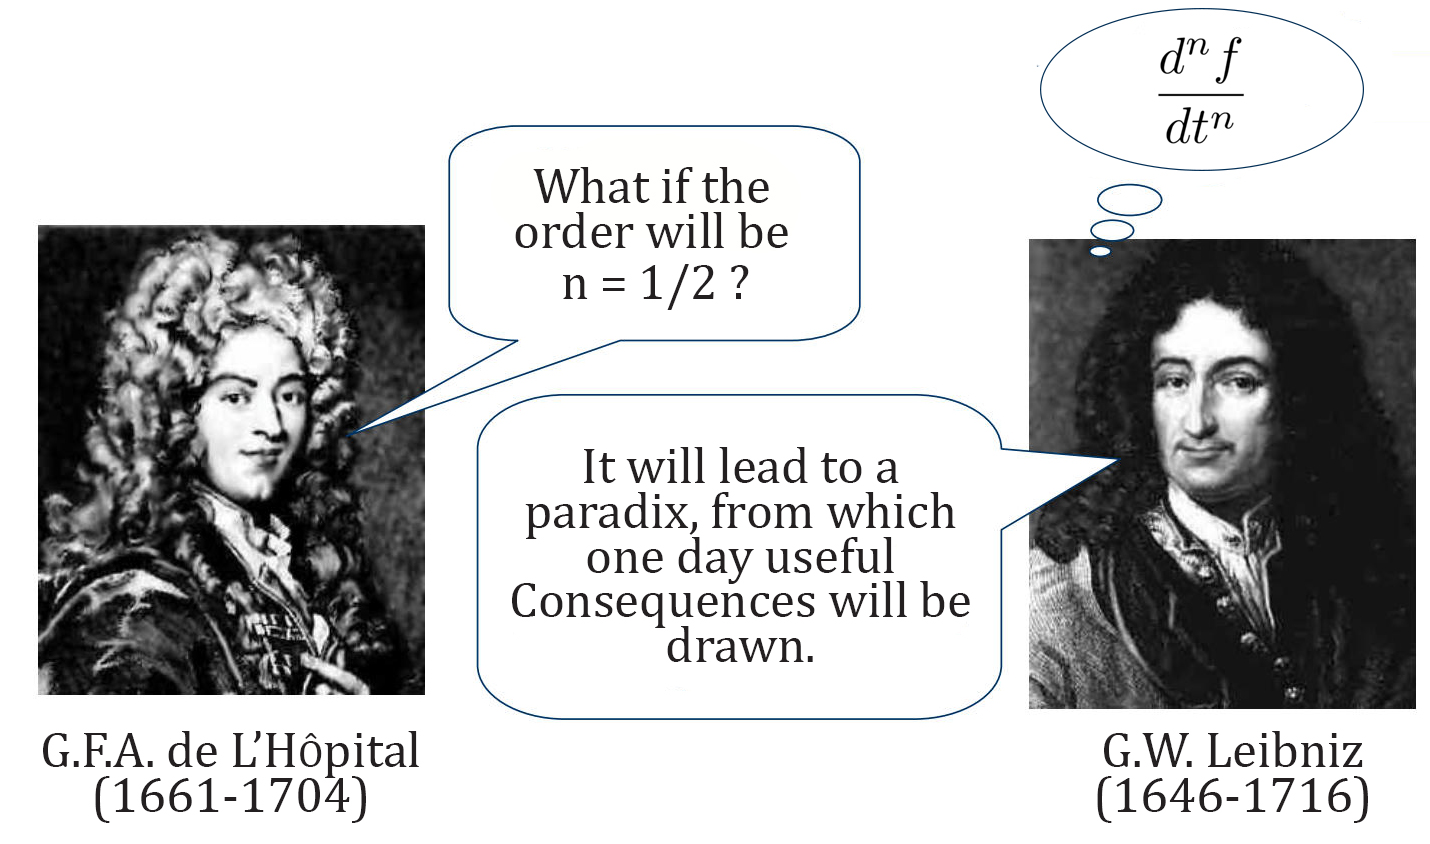
\includegraphics[width=0.9\textwidth]{lei.jpg}\par\vspace{0.5cm}
\end{center}

In his correspondence with Johann Bernoulli, Leibniz mentions derivative of "general order." In Leibniz's correspondence with John Wallis, in which Wallis's infinite product for $\frac{1}{2} \pi$ is discussed, Leibniz states that differential calculus might have been used to achieve this result. He uses the notation $d^{1/2}y$ to denote the derivative of order $\frac{1}{2}$.\\
\newline
The subject of fractional calculus did not escape Euler's attention.\\
In 1730 he wrote: "When  $n$ is positive integer, and if $p$ should be a function of $x$, the ratio $d^{n}p$ to $dx^n$ can always be expressed algebraically, so that if $n=2$ and $p=x^3$, then $d^2 x^3$ to $dx^2$ is $6x$ to $1$.\\ Now it is asked what kind of ratio can then be made if $n$ be a fraction. The difficulty in this case can easily be understood
For if $n$  is a positive integer $d^n$ can be found by continued differentiation. Such a way, however, is not evident if $n$ is a fraction. But yet with the help of interpolation which i have already explained in this dissertation, one may br able to expedite the matter"\\
J. L. Lagrange contributed to fractional calculus indirectly.\\
In 1772 he developed the law of exponents (indices) for differential operators of integer order and wote:
$$\dv[m]{}{x} . \dv[n]{}{x} y = \dv[n+m]{}{x} y$$
In modern notation the dot is omitted, for it is not a multiplication.\\
Later, when the theory of fractional calculus developed, mathematicians were interested in knowing what restrictions has to be imposed on $y(x)$ so that an analogous rule held true for $m$ and $n$ arbitrary.\\
In 1812 P. S. Laplace defined a fractional derivative of arbitrary order appears in a text. S. F. Lacroix devoted less than two pages of his 700-pages text to this topic. He developed a mere mathematical exercise generalizing from a case of integer order. starting with $y=x^m$ , $m$ a positive integer, Lacroix easily develops the $n$th derivative
$$\dv[n]{y}{x} = \frac{m!}{(m-n)!} x^{m-n} , \quad  m \geq n $$
Using Legendre's symbol for the generalized fractional (the gamma function), he generalizations
\begin{equation}
    \label{1.2}
    \dv[n]{y}{x} = \frac{\Gamma{(m+1)}}{\Gamma{(m-n+1)}}x^{m-n}
\end{equation}

He then gives the example for $y=x$ and $n=\frac{1}{2}$, and obtains
$$\dv[1/2]{y}{x} = \frac{2\sqrt{x}}{\sqrt{\pi}}$$

Joseph B. J. Fouriier was the next to mention derivatives of arbitrary order. His definition of fractional operations was obtained from his integral represen-tation of $f(x)$:
$$ f(x) = \frac{1}{2\pi} \int_{-\infty}^{\infty} f(\alpha) d\alpha \int_{-\infty}^{\infty} \cos{(p(x-\alpha))} dp $$
Now
$$\dv[n]{}{x} cos(p(x-\alpha)) = p^n cos[p(x-\alpha) + \frac{1}{2} n \pi]$$
for $n$ an integer. Formally replacing $n$ with $u$ ($u$ arbitrary), he obtains the generalization

$$\dv[u]{}{x} f(x) = \frac{1}{2\pi} \int_{-\infty}^{\infty} f(\alpha) d\alpha \int_{-\infty}^{\infty} p^u cos[p(x-\alpha) + \frac{1}{2}u \pi] dp$$
Fourier states: "The number $u$ that appears in the above will be regarded as any quantity whatsever, positive of negative."\\
\newline
Leibniz, Euler, Laplace, Lacroix and Fourier made mention of derivatives of arbitrary order, but the first use of fractional operations was made by Niels Henrik Abel in 1823. Abel applied the fractional calculus in the solution of an integral equation that arises in the formulation of the tautochrone porblem \footnote{ The problem of determining the shape of the curve such that the time of descent of a frictionless point mass sliding down the curve under the action of gravity is independent of the starting point}. If the time of slide is a known constant, then Abel's integral equation is
\begin{equation}
    \label{ab1}
    k=\int_0^x (x-t)^{-\frac{1}{2}} f(t) dt
\end{equation}
The integral in ($\ref{ab1}$), except for the multiplicative factor $\frac{1}{\Gamma{(\frac{1}{2})}}$, is a particular case of a definite integral that defines fractional integration of order $\frac{1}{2}$. In integral equations such as ($\ref{ab1}$), the function $f$ in the integrand is unknown and is to be determined. Abel wrote the right-hand side of ($\ref{ab1}$) as
$$\sqrt{\pi}[d^{-1/2}/dx^{-1/2}]f(x)$$
Then he operatoed on both sides of the equation with $d^{1/2}/dx^{1/2}$ to obatin
\begin{equation}
    \label{ab2}
    \dv[1/2]{}{x} k = \sqrt{\pi} f(x)
\end{equation}
Because there fractional operators (with suitable condition of $f$) have the property that $D^{1/2}D^{-1/2} f = D^0 f = f$. Thus when the fractional derivative of order $\frac{1}{2}$ of the constant $k$ in ($\ref{ab2}$) is computed, $f(x)$ is determined. This is a remarkable achievement of abel in the fractional calculus. It is important to note that the fractional derivative of a constant is not always equal to zero. It is this curious fact that lies at the center of a mathematical controversy to be discussed shortly.\\
mathematicians have described Abel's solution as "elegant." Perhaps it was Fourier's integral formula and Abel's solution that has attracted the attention of Liouville, who made the first major study of fractional calculus. He publis-\\hed three long memoris in 1832 and several more publications to problems in potential theory\\
The starting point for his theoretical development was the known result for derivatives of integral order:
$$D^m e^{ax} = a^m e^{ax}$$
which he extended in a natural way to derivatives of arbitrary order
$$D^{\nu} e^{ax} = a^{\nu} e^{ax}$$
He assumed that the arbitrary derivative of function $f(x)$ that may be extended in a series of the form
\begin{equation}
    \label{functionclass}
    f(x) = \sum_{n=0}^{\infty} c_n e^{a_n x} , \quad \mathfrak{Re}(a_n) > 0
\end{equation}

is
\begin{equation}
    \label{2.5}
    \mathcal{D}^{\nu}f(x) = \sum_{n=0}^{\infty} c_n a^{\nu}_{n} e^{a_n \nu}
\end{equation}
Formula ($\ref{2.5}$) is known as Liouville's first formula for a fractional derivative. It generalizes in a natural way a derivative of arbitrary order $\nu$, where $\nu$ is any number: rational, irrational, or complex. But it has the obvious disadvantage of being applicable only to functions of he formulated a second definition.\\
To obtain his second definition he strated with a definite integral related to the gamma function:
$$\mathscr{I} = \int_0^\infty u^{a-1} e^{-xu} \, du \quad a>0 \,\, x>0 $$
The change of variable $xu=t$ yields
\begin{align*}
    \mathscr{I} & = x^{-a} \int_0^\infty t^{a-1} e^{-t} \, dt \\
                & = x^{-a} \Gamma{(a)}                        \\
\end{align*}
Or
$$x^{-a} = \frac{1}{\Gamma{(a)}}\mathscr{I}$$
Then Liouvlle operators with $\mathcal{D}^{\nu}$ on both sides of the equation above, to obtain, according to Liouville's basic assumption
$$\mathcal{D}^\nu x^{-a} = \frac{(-1)^\nu}{\Gamma{(a)}} \int_0^\infty u^{a+\nu-1} e^{-xu} \, du$$
Thus Liouville obtains his second definition of a fractionla derivvative:
\begin{equation}
    \label{2.7}
    \mathcal{D}^{\nu} x^{-a} = \frac{(-1)^\nu \gamma{(a+\nu)}}{\Gamma{(a)}} x^{-a-\nu}, \quad a>0
\end{equation}


But Liouville's definitions were too narrow to last. The first definition os restricted to functions of the class ($\ref{functionclass}$), and the second definiton os useful only for functions of the type $x^{-a}$ (with $a>0$). Neither is suitable to be applied to a wide class of functions.\\
\newline
William Center observed that the fractional derivative of a constant, according to the Lacroix-Peacock method, is unequal to zero. Using $x^0$ to denote unity, Center finds the fractional derivative of unity of irder $\frac{1}{2}$, by letting $m=0$ and $n=\frac{1}{2}$ in ($\ref{1.2}$) (even thought Lacroix assumed that $m \geq n$) to obtain
\begin{equation}
    \label{3.1}
    \dv[1/2]{}{x}x^0 = \frac{\Gamma{(1)}}{\Gamma{(\frac{1}{2})}} x^{-1/2} = \frac{1}{\sqrt{\pi x}}
\end{equation}
But as Center points out, according to Liouville's "system"\footnote{referring to Liouville's second defintion goven in formaule ($\ref{2.7}$)}, by letting $a=0$ ( even though Liouville assumed that $a>0$ ), the fractional derivative ofunity equals to zero because $\Gamma{(0)} = \infty $. He continues: "The whole question in plainly reduces to what is $\frac{d^u x^0}{dx^u} $. For when this is determined we shall determine at the same time which is the correct system "\\
Augustus De Morgan devoted three pages to fractional calculus: "Both these systems may very possible be parts of a more general system, but at present I incline to the conclusion that neither system has any claim to be considerer as giving the form $D^n x^m$, though eother may be a form."\\

The state of affairs complained about by De Morgan and Center is now thoroughly cleared up. De Morgan's judgment proved to be correct, for the two systems that Center thought led to irreconcilable results have now been incroporated into a more general system. It is only fair to state that mathematicians at that time were aiming for a plausible defintion of generali-\\zed integration and differentiation.\\
\newline
Liouville and Later C. J. Hargreave wrote on the generalixation of Leibniz' nth derivative of a product when n is not a positive integr. In modern form
$$\mathcal{D}^{\nu}f(x) g(x) = \sum_{n=0}^{\infty} {\nu \choose n} \mathcal{D}^n f(x) \mathcal{D}^{\nu-n}g(x) $$
Where $\mathcal{D}^n$ is the ordinary differentiation operator of order $n$, $\mathcal{D}^{\nu -n}$ a fractional operator, and ${\nu \choose n}$ the generalized bionomial coefficient $\frac{\Gamma{(\nu+1)}}{n! \Gamma{(\nu-n+1)}}$. The general-\\ized Leibniz rule may be found in many modern applications H. R. Greer wrote on finite differences of fractional order. Surprisingly, a recent access to a fractional derivative is by means of finite differences. Mention should also be made of a paper by W. Zachartchenxo. He imporoves on the work of Greer, and he ends his paper with an amusing note, which no modern amthematiciam would admit. Concerning his research on a topic: "I konw that Liouville, peacock and Kelland have written on this topci, but i have had no opportunity to read their works." H. Holmgren wrote a long monograph on the application of fractional calculus to the solution of cartain ordinary differential equations. In the introduction to this work as his point of departure, states that his aim in this paper is to find a complete solution not subject to the restrictions on the independent variable that his predecessors has made. He proceeds along formal lines. For example, the index law is used:
$$\mathcal{D}^\nu y^{''} = \mathcal{D}^\nu \mathcal{D}^2 y= \mathcal{D}^{\nu+2}y$$
Although his rule is valid for $\nu$ a positive integer, modern mathematicians would seek to justify this rule when $\nu$ is arbitrary

Finally, After many developments, By the second half of the twentieth century, the field of fractional calculus had grown to such extent that in
1974 the first conference “The First Conference on Fractional Calculus and its Applications” concerned solely
with the theory and applications of fractional calculus was held in New Haven. In the same year, the first book
on fractional calculus by Oldham and Spanier was published after a joint collaboration started in 1968\\

A number of additional books have appeared since then, for example Mc-Bride (1979), Nishimoto (1991)
, Miller and Ross (1993), etc \\
In 1998 the first issue of
the mathematical journal “Fractional calculus and applied analysis” was printed. This journal is solely
concerned with topics on the theory of fractional calculus and its applications. Finally, in 2004 the first
conference “Fractional differentiation and its applications” was held in Bordeaux, and it is organized every
second year since 2004.



\vspace{3em}
This research is organized as follows.\\
Chapter 2 on imporant Preliminaries, Chapter 3 Review of fractional derivatives definitions, chapter 4 Disscusion on fractional derivatives with non-singular (bounded) kernels ,their definiton ,propoerties and drawbacks, and finally chapter 5 Introduction to Fractional Differential Equations with non-singular kernel derivatives and on Existence and uniquesness theorems
%==========================================================
\chapter{Preliminaries}

\section*{Special functions}
\subsection*{Gamma Function}
We start by considering the Gamma function which is denoted by $\Gamma{(.)}$ is defined as:
$$\Gamma{(n)} := \int_0^\infty e^{-t}t^{n-1} dt $$
\subsubsection*{Properties of Gamma function}
Function $\Gamma{(n)}$ is convergent for $n>0$ and consequently is divergent for $n \leq 0$\\
Gamma function obeys the property:
$$\Gamma{(n+1)} = n \Gamma{(n)}$$
For Integer inputs of this function it could be treated as usual factorial function
$$\Gamma{(n+1)} = n! \quad n \text{  is integer}$$
\subsection*{Mittag-Leffler Function}
In this section we introduce the one- and two-parameter Mittag-Leffler functions, denoted as $E_\alpha (.)$ and $E_{\alpha ,\beta} (.)$ respectilvely.
$$E_\alpha (z) = \sum_{k=0}^\infty \frac{z^k}{\Gamma{(\alpha k +1)}} \quad \mathfrak{Re}(\alpha) > 0$$
$$E_{(\alpha,\beta)}(z) := \sum_{k=0}^\infty \frac{z^k}{\Gamma{(\alpha k +\beta)}}  \quad \mathfrak{Re}(\alpha) > 0 , \mathfrak{Re}(\beta) > 0$$

One of important properties is that
$$\Laplace\{E_{\alpha}\left(-\lambda t^{\alpha}\right)\} = \frac{p^{\alpha -1}}{s^{\alpha} + \frac{\alpha}{1-\alpha}}$$

\section*{$L_p$ Spaces}
\begin{center}
    \begin{tikzpicture}
        \draw (0,0) ellipse (3cm and 2.3cm);
        \draw (0,2.12) node{$L_1$};
        \draw (0,0) ellipse (2.13 cm and 1.9cm);
        \draw (0,1.7) node{$L_2$};
        \draw (0,1.35) node{$\vdots$};
        \draw (0,0) ellipse (1cm and 1 cm);
        \draw (0,0.7) node{$C$};
        \draw (0,0) ellipse (0.45cm and 0.45 cm);
        \draw (0,0) node{$AC$};
    \end{tikzpicture}
\end{center}
We introduce some important definitions\\
\Definition{
\textbf{$L_p$ Spaces} Let $\mathfrak{u} \in \Omega_L$. The $L_p(\mathfrak{u}), p\geq 1$ space consisting of all measurable functions $f$, with the property that
$$\left(\int_\mathfrak{u} |f(x)|^p dx\right)^{\frac{1}{p}} < \infty , p\in[1,\infty) \text{ and } ess\,\,sup_{x\in\mathfrak{u}} |f(x)| < \infty , p =\infty$$
}
\Definition{
    \textbf{Absolute Continuous functions} By $AC^{n}[\Omega] , n \in \mathbb{N}:=\{1,2,3,\dots\}$, we denotes the space of functions $f$ defined on $[0,b]$ which have continuous derivatives up to order $n-1$ on $[0,b]$ with $f^{(n-1)}$ is absolutely continuous $[\Omega]$
    $$AC^n(\Omega)=\{f :  f^{(i)}\in C(\Omega) \forall i=1,2,\dots,(n-1) \text{and} f^{(n-1)}(x) \in AC(\Omega) \} $$
}
Here is an important theorem about Absolute continuous functions
\Theorem{\\
If $f : [a,b] \rightarrow \mathbb{R}$ is absolutely continuous, then $f$ is differentiable a.e. in $[a,b]$, $f' \in L^{1}(a,b)$, and
$$f(x) = f(a) + \int_a^x f'(t) dt \qquad \forall x \in [a,b]$$
}


\Definition{  \textbf{Sobolev Space of order 1}\\
    The sobolev space is defined easily as follows. The sobolev space of order 1 denoted by $H^1$
    $$H^1(a,b) = \{ u \in L^2(a,b) \, | \, u' \in L^2(a,b)  \} $$
}


%===========================================================================================
\chapter{How Many Fractional Derivatives Are There ?}
In this chapter we consider the most important definitions of fractional derivatives [10,18]
\begin{itemize}
    \item Liouville derivative
          \begin{equation}
              \mathcal{D}^{\alpha}[f(x)] = \frac{1}{\Gamma{(1-\alpha)}} \dv{}{x} \int_{-\infty}^x (x-\xi)^{-\alpha} f(\xi) d\xi \, , \quad -\infty< x <+\infty
          \end{equation}

    \item Liouville left-sided derivative
          \begin{equation}
              \mathcal{D}^{\alpha}_{0+}[f(x)] = \frac{1}{\Gamma{(n-\alpha)}} \dv[n]{}{x} \int_0^x (x-\xi)^{-\alpha+n-1} f(\xi) d\xi  \,\, , x >0
          \end{equation}
    \item Liouville right-sided derivative
          \begin{equation}
              \mathcal{D}^{\alpha}_{-}[f(x)] = \frac{(-1)^n}{\Gamma{(n-\alpha)}} \dv[n]{}{x} \int_x^\infty (x-\xi)^{-\alpha+n-1} f(\xi) d\xi  \,\, ,  x <\infty
          \end{equation}

    \item Riemann-Liouville left-sided derivative
          \begin{equation}
              ^{Rl}\mathcal{D}^{\alpha}_{a+}[f(x)] = \frac{1}{\Gamma{(n-\alpha)}} \dv[n]{}{x} \int_a^x (x-\xi)^{n-\alpha+1} f(\xi) d\xi  \,\, ,   x \geq a
          \end{equation}

    \item Riemann-Liouville right-sided derivative
          \begin{equation}
              ^{Rl}\mathcal{D}^{\alpha}_{b-}[f(x)] = \frac{(-1)^n}{\Gamma{(n-\alpha)}} \dv[n]{}{x} \int_x^b (\xi-x)^{n-\alpha+1} f(\xi) d\xi  \,\, ,   x \leq b
          \end{equation}
    \item Caputo left-sided derivative
          \begin{equation}
              _{*}\mathcal{D}^{\alpha}_{a+}[f(x)] = \frac{1}{\Gamma{(n-\alpha)}} \int_a^x (x-\xi)^{n-\alpha-1} \dv[n]{}{\xi}[f(\xi)] d\xi  \,\, , x \geq a
          \end{equation}
    \item Caputo right-sided derivative
          \begin{equation}
              _{*}\mathcal{D}^{\alpha}_{b-}[f(x)] = \frac{(-1)^n}{\Gamma{(n-\alpha)}} \int_x^b (\xi-x)^{n-\alpha-1} \dv[n]{}{\xi}[f(\xi)] d\xi  \,\, , x \leq b
          \end{equation}
    \item Gr$\ddot{u}$nwald-Letnikov left-sided derivative
          \begin{equation}
              ^{Gl}\mathcal{D}^{\alpha}_{a+}[f(x)] = \lim_{h\to 0} \frac{1}{h^\alpha} \sum_{k=0}^{\lfloor n \rfloor} (-1)^k \frac{\Gamma{(\alpha+1) f(x-kh)}}{\Gamma{(k+1)} \Gamma{(\alpha-k+1)}} \,\, , nh=x-a
          \end{equation}
    \item Gr$\ddot{u}$nwald-Letnikov right-sided derivative
          \begin{equation}
              ^{Gl}\mathcal{D}^{\alpha}_{b-}[f(x)] = \lim_{h\to 0} \frac{1}{h^\alpha} \sum_{k=0}^{\lfloor n \rfloor} (-1)^k \frac{\Gamma{(\alpha+1) f(x+kh)}}{\Gamma{(k+1)} \Gamma{(\alpha-k+1)}} \,\, , nh=b-x
          \end{equation}
    \item Weyl derivative
          \begin{equation}
              _{x}\mathcal{D}^{\alpha}_{\infty}[f(x)] = \mathcal{D}^{\alpha}_{-}[f(x)] = (-1)^m \left(\dv{}{\xi}\right)^n \left[_{x}W^{\alpha}_{\infty}[f(x)]\right]
          \end{equation}
    \item Marchaud derivative
          \begin{equation}
              \mathcal{D}^{\alpha}[f(x)]=\frac{\alpha}{\Gamma{(1-\alpha)}} \int_{-\infty}^x \frac{f(x)-f(\xi)}{(x-\xi)^{1+\alpha}} d\xi
          \end{equation}
    \item Marchaud left-sided derivative

          \begin{equation}
              \mathcal{D}^{\alpha}_{+}[f(x)]=\frac{\alpha}{\Gamma{(1-\alpha)}} \int_0^\infty \frac{f(x)-f(x-\xi)}{\xi^{1+\alpha}} d\xi
          \end{equation}
    \item Marchaud right-sided derivative

          \begin{equation}
              \mathcal{D}^{\alpha}_{-}[f(x)]=\frac{\alpha}{\Gamma{(1-\alpha)}} \int_0^\infty \frac{f(x)-f(x+\xi)}{\xi^{1+\alpha}} d\xi
          \end{equation}
    \item Hadamard derivative
          \begin{equation}
              \mathcal{D}^{\alpha}_{+} = \frac{\alpha}{\Gamma{(1-\alpha)}} \int_0^x \frac{f(x)-f(\xi)}{[\ln{(\frac{x}{\xi})}]^{1+\alpha}} \frac{d\xi}{\xi}
          \end{equation}
    \item Chen left-sided derivative
          \begin{equation}
              \mathcal{D}^{\alpha}_{c} [f(x)] = \frac{1}{\Gamma{(1-\alpha)}} \dv{}{x} \int_c^x  (x-\xi)^{-\alpha} f(\xi) d\xi \,\, , x>c
          \end{equation}
    \item Chen right-sided derivative
          \begin{equation}
              \mathcal{D}^{\alpha}_{c}[f(x)] = \frac{-1}{\Gamma{(1-\alpha)}} \dv{}{x} \int_x^c  (\xi-x)^{-\alpha} f(\xi) d\xi \,\, , x<c
          \end{equation}
    \item Davidson-Essex derivative
          \begin{equation}
              \mathcal{D}^{\alpha}_{0}[f(x)] = \frac{1}{\Gamma{(1-\alpha)}} \dv[n+1-k]{}{x} \times \int_0^x (x-\xi)^{\alpha} \dv[k]{}{\xi}[f(\xi)] d\xi
          \end{equation}
    \item Coimbra derivative
          \begin{equation}
              \mathcal{D}^{\alpha(x)}_{0}[f(x)] = \frac{1}{\Gamma{(1-\alpha(x))}} \times \left( \int_0^x (x-\xi)^{-\alpha(x)} \dv{}{\xi} [f(x)] d\xi + f(0) x^{-\alpha(x)} \right)
          \end{equation}
    \item Canavati derivative
          \begin{equation}
              _{a}\mathcal{D}^{\nu}_{x}[f(x)] = \frac{1}{\Gamma{(1-\mu)}} \dv{}{x} \int_0^x (x-\xi)^\mu \dv[n]{}{\xi} [f(\xi)] d\xi \,\, , n= \lfloor \nu \rfloor \,, \mu=n-\nu
          \end{equation}
    \item Jumarie derivative , $n=1$
          \begin{equation}
              \mathcal{D}^{\alpha}_{x}[f(x)] = \frac{1}{\Gamma{(n-\alpha)}} \dv[n]{}{x} \times \int_0^x (x-\xi)^{n-\alpha-1}[f(\xi)-f(0)] d\xi
          \end{equation}

    \item Riesz derivative
          \begin{equation}
              \begin{split}
                  \mathcal{D}^{\alpha}_{x}[f(x)] & = - \frac{1}{2 \cos{(\frac{\alpha \pi}{2})}} \frac{1}{\Gamma{(\alpha)}}                                                                     \\
                                                 & \quad \times \dv[n]{}{x} \left( \int_{-\infty}^{x} (x-\xi)^{n-\alpha-1} f(\xi) d\xi + \int_x^\infty (\xi-x)^{n-\alpha-1}f(\xi) d\xi \right)
              \end{split}
          \end{equation}
    \item Cossar derivative
          \begin{equation}
              \mathcal{D}^{\alpha}_{-}[f(x)] = - \frac{1}{\Gamma{(1-\alpha)}} \lim_{N \to \infty} \dv{}{x} \int_x^N (\xi-x)^{-\alpha} f(\xi) d\xi
          \end{equation}
    \item Local fractional Yang derivative
          \begin{equation}
              \mathcal{D}^{\alpha}_{-}[f(x)]|_{x=x_0} = \lim_{x \to x_0} \frac{\Delta^\alpha [f(x)-f(x_0)]}{(x-x_0)^\alpha}
          \end{equation}
    \item Left Riemann-Liouville derivative of variable fractional order
          \begin{equation}
              _{a}\mathcal{D}^{\alpha(.,.)}_{x}[f(x)] = \dv{}{x} \int_a^x (x-\xi)^{-\alpha(\xi,x)} f(\xi)\frac{d\xi}{\Gamma{[1-\alpha(\xi,x)]}}
          \end{equation}
    \item Right Riemann-Liouville derivative of variable fractional order
          \begin{equation}
              _{x}\mathcal{D}^{\alpha(.,.)}_{b}[f(x)] = \dv{}{x} \int_x^b (\xi-x)^{-\alpha(\xi,x)} f(\xi)\frac{d\xi}{\Gamma{[1-\alpha(\xi,x)]}}
          \end{equation}
    \item Left Caputo derivative of variable fractional order
          \begin{equation}
              _{a}\mathcal{D}^{\alpha(.,.)}_{x}[f(x)] = \int_a^x (x-\xi)^{-\alpha(\xi,x)} \dv{}{\xi} f(\xi)\frac{d\xi}{\Gamma{[1-\alpha(\xi,x)]}}
          \end{equation}
    \item Right Caputo derivative of variable fractional order
          \begin{equation}
              _{x}\mathcal{D}^{\alpha(.,.)}_{b}[f(x)] = \int_x^b (\xi-x)^{-\alpha(\xi,x)} \dv{}{\xi} f(\xi)\frac{d\xi}{\Gamma{[1-\alpha(\xi,x)]}}
          \end{equation}
    \item Caputo derivative of variable fractional order
          \begin{equation}
              _{*}\mathcal{D}^{\alpha(x)}_{x}[f(x)] = \frac{1}{\Gamma{(1-\alpha(x))}} \int_0^x (x-\xi)^{-\alpha(\xi,x)} \dv{}{\xi} f(\xi) d\xi
          \end{equation}
    \item Modified Riemann-Liouville fractional derivative
          \begin{equation}
              \mathcal{D}^{\alpha}[f(x)] = \frac{1}{\Gamma{(1-\alpha)}} \dv{}{x} \int_0^x (x-\xi)^{\alpha} [f(\xi)-f(0)] d\xi
          \end{equation}
    \item Osler fractional derivative
          \begin{equation}
              _{a}\mathcal{D}^{\alpha}_{z} [f(z)] = \frac{\Gamma{(\alpha+1)}}{2\pi i} \int_{\mathcal{C}(a,z^+)} \frac{f(z)}{(\xi-z)^{1+\alpha}} d\xi
          \end{equation}
    \item K-fractional Hilfer derivative
          \begin{equation}
              ^{k}\mathcal{D}^{\mu,\nu} f(x) = I^{\nu(1-\mu)}_k \dv{}{x} I^{(1-\mu)(1-\nu)}_k f(x)
          \end{equation}

    \item Gohar fractional derivative
          \begin{equation}
              G_{\alpha} f(x) = \lim_{h \to 0 } \frac{f\left( x \left[ 1+ \ln{(1+h \frac{\Gamma{(n)}}{\Gamma{(n-\alpha+1)}}) x^{\alpha}}\right]\right) - f(x)}{h}
          \end{equation}
\end{itemize}


%===========================================================================================
\chapter{Derivatives with non-singular kernels}
Now, we introduce a simple discussion on derivatives with non-singular kernels, properties and their drawbacks
\section{Caputo-Fabrizio Type}
Let us recall the usual Caputo fractional derivative of order $\alpha$, given by
\begin{equation}
    \label{UsualD}
    ^{C}\mathcal{D}^{\alpha}_{a+} f(t) = \frac{1}{\Gamma{(1-\alpha)}} \int_a^t (t-\xi)^{-\alpha} \dv{}{\xi}f(\xi)d\xi
\end{equation}
with $\alpha \in [0,1)$ and $a \in (-\infty ,t) \, , f \in H^1(a,b) \, ,b>a$. By changing the kernel $(t-\xi)^{-\alpha}$ with the function $\exp(- \frac{\alpha}{1-\alpha}(t-\xi))$ and $\frac{1}{\Gamma{(1-\alpha)}}$ by $\frac{M(\alpha)}{1-\alpha}$, we obtain the following new definition of fractional derivative
\Definition{\\
    Let $f \in H^1(a,b), b>a , \alpha \in [0,1]$, then, the Caputo-Fabrizio derivative with order $\alpha$ is defined as:
    \begin{equation}
        \label{NewD}
        ^{CF}\mathcal{D}^{\alpha}_{a+}f(t) = \frac{M(\alpha)}{1-\alpha} \int_a^t \exp(- \frac{\alpha (t-\xi)}{1-\alpha}) \dv{f(\xi) }{\xi}d\xi
    \end{equation}
}

where $M(\alpha)$ is a normalization function such taht $M(0)=M(1)=1$. According to the new definition ($\ref{NewD}$) The new fractional derivative is zero when $f(t)$ is constant, as in the usual definiton ($\ref{UsualD}$), but contrary to the usual definition, the kernel does not have singularity for $t=\xi$\\
The new definition can also be applied to functions that do not belong to $H^1(a,b)$. Indeed, the definition ($\ref{NewD}$) can be formulated also for $f \in L^1(a,b)$
\begin{equation}
    \label{NewD-Case}
    ^{CF}\mathcal{D}^{\alpha} f(t) = \frac{\alpha M(\alpha)}{1-\alpha} \int_{a}^{t} (f(t)-f(\xi)) \exp(-\frac{\alpha(t-\xi)}{1-\alpha})d\xi
\end{equation}
Now, it is worth to observe that if we put
$$\sigma = \frac{1-\alpha}{\alpha} \in [0,\infty] \,\, , \,\, \alpha = \frac{1}{1+\sigma} \in [0,1] $$
The definition ($\ref{NewD}$) can be written as
\begin{equation}
    \label{NewD-sigma}
    ^{CF}\tilde{\mathcal{D}}^{\sigma} f(t) = \frac{N(\sigma)}{\sigma} \int_a^t \dv{f(\xi) }{\xi}\exp(-\frac{(t-\xi)}{\sigma}) d\xi
\end{equation}
Where $\sigma \in [0,\infty]$ and $N(\sigma)$ is the corresponding normalization term of $M(\alpha)$, such that $N(0)=N(\infty) = 1$. Moreover, because
\begin{equation}
    \lim_{\sigma \to 0} \frac{1}{\sigma} \exp(-\frac{(t-\xi)}{\sigma}) = \delta(t-\xi)
\end{equation}
and for $\alpha \to 1$, we have $\sigma \to 0$. Then
\begin{align*}
    \lim_{\alpha \to 1} {^{CF}\mathcal{D}^{\alpha}} f(t) & = \lim_{\alpha \to 1} \frac{M(\alpha)}{1-\alpha} \int_a^t \dv{f(\xi)}{\xi} \exp(- \frac{\alpha(t-\xi)}{1-\alpha}) d\xi       \\
                                                         & = \lim_{\sigma \to 0 } \frac{N(\sigma)}{\sigma}  \int_a^t \dv{f(\xi)}{\xi} \exp(-\frac{(t-\xi)}{\sigma}) d\xi = \dv{f(t)}{t}
\end{align*}
Otherwise, when $\alpha \to 0$, then $\sigma \to +\infty$. Hence,
\begin{align*}
    \lim_{\alpha \to 0} {^{CF}\mathcal{D}^{\alpha}} f(t) & = \lim_{\alpha \to 0} \frac{M(\alpha)}{1-\alpha} \int_a^t \dv{f(\xi)}{\xi} \exp(-\frac{\alpha(t-\xi)}{1-\alpha}) d\xi           \\
                                                         & = \lim_{\sigma \to +\infty} \frac{N(\sigma)}{\sigma} \int_a^t \dv{f(\xi)}{\xi} \exp(-\frac{(t-\xi)}{\sigma}) d\xi = f(t) - f(a) \\
\end{align*}
\Remark{$$\int_{-\infty}^{\infty} f(\theta) \delta(t-\theta) d\theta = f(t) $$ for any $f(\theta)$ continuous at $t$}
Also, If $n\geq 1$, and $\alpha \in [0,1]$ the fractional derivative $\mathcal{D}^{(\alpha +n )} f(t)$ of order $(n+\alpha)$ is defined by
\begin{equation}
    \label{a2.8}
    \mathcal{D}^{(\alpha +n )} f(t) := \mathcal{D}^{\alpha}(\mathcal{D}^{n} f(t))
\end{equation}
\Theorem{\\
    For new fractional derivative, if the function $f(t)$ is such that
    $$f^{(s)}(a) = 0 , \qquad s=1,2,\dots,n$$
    Then we have
    \begin{equation}
        \label{a2.9}
        \mathcal{D}^{n}(\mathcal{D}^{\alpha} f(t)) = \mathcal{D}^{\alpha} (\mathcal{D}^{n} f(t))
    \end{equation}
}
\begin{proof}
    We bagin considering $n=1$, then from defintion ($\ref{a2.8}$) of $\mathcal{D}^{\alpha +1} f(t)$ we obtain

    \begin{equation}
        \label{a2.10}
        \mathcal{D}^{\alpha} (\mathcal{D}^{1} f(t)) = \frac{M(\alpha)}{1-\alpha} \int_a^t \ddot{f}(\xi) \exp\left[ - \frac{\alpha(t-\xi)}{1-\alpha} \right] d\xi
    \end{equation}
    Hence, after an integration by parts and assuming $f'(a) = 0$, we hhave
    \begin{align*}
        \mathcal{D}^{\alpha}(\mathcal{D}^{1} f(t)) & = \frac{M(\alpha)}{1-\alpha} \int_a^t  \ddot{f}(\xi) \exp\left[- \frac{\alpha(t-\xi)}{1-\alpha}\right] d\xi                                                                                                   \\
                                                   & = \frac{M(\alpha)}{1-\alpha}\left[ \exp(-\frac{\alpha(t-\xi)}{1-\alpha}) \dot{f}(t)|_{a}^{t} +\frac{\alpha }{1-\alpha} \int_a^t (\dot{f}(\xi) \exp\left[ -\frac{\alpha(t-\xi)}{1-\alpha} \right] d\xi \right] \\
                                                   & = \frac{M(\alpha)}{1-\alpha} \left[\dot{f}(t) +\frac{\alpha}{1-\alpha} \mathcal{D}^{\alpha}f(t)\right]
    \end{align*}
    Similarly
    $$\mathcal{D}^{1}(\mathcal{D}^{\alpha}f(t)) = \frac{M(\alpha)}{1-\alpha} \left[\dot{f}(t) +\frac{\alpha}{1-\alpha} \mathcal{D}^{\alpha}f(t) \right]$$
    It is easy to generalize the proof for any $n>1$
\end{proof}

Now after the introduction of a new derivative, the associate anti-derivative becomes important, the associated integral of the new Caputo derivative with fractional order was proposed by Losada and Nieto
\Definition{\\
    Let $0<\alpha<1$. the fractional integral of order $\alpha$ of a function $f$ is defined By
    \begin{equation}
        \mathscr{I}^{\alpha} f(t) = \frac{2(1-\alpha)}{(2-\alpha)M(\alpha)}f(t) + \frac{2\alpha}{(2-\alpha) M(\alpha)}\int_0^t f(s) ds ,\,\, t\geq0
    \end{equation}
}
On the other hand, we discuss Caputo-Fabrizio in Riemann-Liouville Sense
\Definition{\\
    Let $f$ be a function not necessarily differential, Let $\alpha$ be a real number such that $0 \leq \alpha \leq 1$, then the Caputo-Fabrizio derivative in Riemann sense with order $\alpha$ is given as:
    \begin{equation}
        \label{newdef-riemann}
        ^{CR}\mathcal{D}^{\alpha}_{a+} f(t) = \frac{1}{1-\alpha} \dv{}{t} \int_a^t f(\xi) \exp\left[-\alpha \frac{t-\xi}{1-\alpha}\right] d\xi
    \end{equation}

}
If $\alpha$ is zero, we have the following
$$^{CR}\mathcal{D}^{0} f(t) = \dv{}{t} \int_a^t f(\xi) d\xi = f(t)$$
Using the argument by Caputo and Fabrizio, we also have that when $\alpha \rightarrow 1$, we recover the first derivative.

The last two definitions Caputo Fabrizio and Caputo in Riemann sense can be connected as follows
\Theorem{\\
    The Caputo-Fabrizio derivative with fractional order is connected to the CR derivative as follows:
    \begin{equation}
        \label{5.118}
        \theta(\alpha) ^{CF}\mathcal{D}^{\alpha} (f(t)) = \theta(\alpha) ^{CR}\mathcal{D}^{\alpha}(f(t)) + f(0)\exp(-f(\alpha)x)
    \end{equation}
    Where
    $$\theta(\alpha) = \frac{1-\alpha}{M(\alpha)} \qquad f(\alpha)= \frac{\alpha}{1-\alpha}$$
}
\begin{proof}
    By definition, we have the following:
    \begin{align*}
        \theta(\alpha) ^{CF}\mathcal{D}^{\alpha} (f(t)) & = \dv{}{x} \int_0^t h(y) \exp(-f(\alpha)(t-y))dy                                                  \\
                                                        & = h(t) - f(\alpha) \int_0^t h(y) \exp(-f(\alpha)(t-y))dy                                          \\
                                                        & = h(y) - f(\alpha)\left[\frac{h(t)}{f(\alpha)} - \frac{h(0)}{f(\alpha)}\exp(-f(\alpha)t)  \right. \\
                                                        & \left. - \frac{1}{f(\alpha)}\int_0^t \exp(-f(\alpha)(t-y))dy \right]                              \\
                                                        & = \frac{h(0)}{f(\alpha)}\exp(-f(\alpha)t)+\int_0^t \dv{h(y)}{t}\exp(-f(\alpha)(t-y))dy            \\
                                                        & = \theta(\alpha) ^{CR}\mathcal{D}^{\alpha}f(t) + f(0)\exp(-f(\alpha)x)
    \end{align*}
    This completes the proof.
\end{proof}
\section{Atangana-Baleanu}
The derivative introduced by Caputo cannot produce the original function when $\alpha$ is zero. How ever this issue was, so far, independently solved by Atangana with Goufo and Caputo with Fabrizio, Respectively\\
Some issues [9] were pointed out against the Caputo-Fabrizio derivative with fractional order:
\begin{itemize}
    \item The kernal used in the Caputo-Fabrizio derivative is Local
    \item The anti-derivative associated to their derivatives is not a fractional integral but the average of the function and its integral
    \item When the fractional order is zero we do not recover the initial (original) function
\end{itemize}
It appears that such a used kernel cannot be used for many physical problems. Therefore, for
a given data we ask the following question: What is the most accurate kernel which better
describes it? Then Atangana and Baleanu suggested a possible answer, presented in the following discussion.\\
\newline
The exponential function is the solution of the following ordinary differential equation:
\begin{equation}
    \dv{y}{x} = a\, y
\end{equation}
However, the Mittag-Leffler function os a solution of the following fractional ordinary differential equation:
\begin{equation}
    \mathcal{D}^{\alpha} (y) = a \, y \quad 0<\alpha<1
\end{equation}
The mittag-Leffler function and ots generalized versions are therefore consided as non-local functions. let us consider the following generalized Mittag-Leffler function:
\begin{equation}
    E_{\alpha}(-t^\alpha) = \sum_{k=0}^{\infty} \frac{(-t)^{\alpha k}}{\Gamma{( \alpha k +1)}}
\end{equation}
The above function has the following properties
\begin{equation}
    E_{1}(-t) = \sum_{k=0}^{\infty} \frac{(-t)^{ k}}{\Gamma{ (k +1)}} = \exp(-t)
\end{equation}
The Taylor series of $\exp(-a(t-y))$ is given by:
\begin{equation}
    \exp(-a(t-y))  = \sum_{k=0}^{\infty} \frac{(-a(t-y))^k}{k!}
\end{equation}
Chosing $a = \frac{\alpha}{1-\alpha}$ and replacing the above expression into Caputo-Fabrizio derivative, the following formula is obtained:
\begin{equation}
    ^{C}\mathcal{D}^{\alpha} f(t) = \frac{M(\alpha)}{1-\alpha} \int_b^t f'(\xi) \sum_{k=0}^{\infty}  \frac{(-a(t-\xi))^k}{k!} d\xi
\end{equation}
Rearranging, they obtained
\begin{equation}
    \label{1}
    ^{C}\mathcal{D}^{\alpha} f(t) = \frac{M(\alpha)}{1-\alpha} \sum_{k=0}^{\infty} \frac{(-a)^k}{k!} \int_b^t f'(\xi)   (t-\xi)^k d\xi
\end{equation}
To solve the problem of non-locality, they derived the following expression. in equation ($\ref{1}$) they replaced $k!$ by $\Gamma{(\alpha k +1)}$ and  $(t-\xi)^k$ by $(t-\xi)^{\alpha k}$ to obatin
\begin{equation}
    \label{AB}
    ^{AB}\mathcal{D}^{\alpha} f(t) = \frac{M(\alpha)}{1-\alpha} \sum_{k=0}^\infty \frac{(-a)^{k}}{\Gamma{(\alpha k +1)}} \int_b^t f'(\xi) (t-\xi)^{\alpha k}  d\xi
\end{equation}
Then the following derivative proposed

\Definition{\\
    Let $f \in H^1(a,b) \, ,b>a \, ,\alpha \in [0,1]$, Then the definition of the Atangana-Baleanu derivative in caputo sense is given as:
    \begin{equation}
        \label{atangana derivative C}
        ^{ABC}_{a}\mathcal{D}^{\alpha} f(t) = \frac{B(\alpha)}{1-\alpha} \int_a^t \dv{f(\xi)}{\xi} E_{\alpha}\left[ -\alpha \frac{(t-\xi)^\alpha}{1-\alpha} \right] d\xi
    \end{equation}
}
Of course $B(\alpha)$ has the same properties as in Caputo and Fabrizio case. The above definition will be helpful to real-world problems and also will have a great advantage when usgine Laplace Transform to solve some physical problems with initial conditions. However, when $\alpha$ is $0$ we do not recover the originl function except when at the origin the function vanished.\\
\newline
To avoid this issue, we propose the following definiton such that researchers in the field of fractional calculus have a choice when dealing with a given problem  \\
\Definition{\\
    Let $f \in H^1(a,b) \, ,b>a \, ,\alpha \in [0,1]$, Then the definition of the Atangana-Baleanu derivative in Riemann-Liouville sense is given as:
    \begin{equation}
        \label{atangana derivative RL}
        ^{ABR}_{b}\mathcal{D}^{\alpha} f(t) = \frac{B(\alpha)}{1-\alpha}\dv{}{t} \int_b^t f(\xi) E_{\alpha}\left[ -\alpha \frac{(t-\xi)^\alpha}{1-\alpha} \right] d\xi
    \end{equation}
}
Equations ($\ref{atangana derivative C}$) and ($\ref{atangana derivative RL}$) have non-local kernels\\
Also equation ($\ref{atangana derivative C}$) when the function is constant the fractional derivative produces zero. Now, we discuss some important Properties\\
\begin{enumerate}
    \item
          \begin{equation}
              \label{laplace-Cap}
              \Laplace\{^{ABC}_{a}\mathcal{D}^{\alpha} x(t)\} = \frac{B(\alpha)}{1-\alpha} \, \frac{p^{\alpha}\Laplace\{x(t)\} - p^{\alpha -1} x(a)}{p^\alpha +  \frac{\alpha}{1-\alpha} }
          \end{equation}
    \item
          \begin{equation}
              \label{laplace-Rie}
              \Laplace\{^{ABR}_{a}\mathcal{D}^{\alpha} x(t)\} = \frac{B(\alpha)}{1-\alpha} \, \frac{p^{\alpha}\Laplace\{x(t)\} }{p^\alpha +  \frac{\alpha}{1-\alpha} }
          \end{equation}
\end{enumerate}

\Definition{\\
The associated fractional integral is defined by
$$^{AB}_{a}\mathscr{I}^{\alpha} x(t) = \frac{1-\alpha}{B(\alpha)} x(t) + \frac{\alpha}{B(\alpha)} (_{a}\mathscr{I}^{\alpha} x(t))$$
Where $(_{a}\mathscr{I}^{\alpha})$ is the left Riemann-Liouville fractional integral
}

\section{Drawbacks of non-singular kernel}
At first sight, fractional derivatives defined using non-sigular (i.e bounded) kernels may appear very attractive since they avoid several difficulties that are caused by the singular nature of the RL and Dzhrbashyan-Caputo kernel.[11]\\


Caputo type derivatives that are defined using nonsingular kernels must fails to satisfy the fundamental theorem of fractional calculus. In other words they don't allow the existence of a corresponding convolution integral for which the derivative is left-inverse\\
\newline
\Theorem{\textbf{(The fundamental theorem of fractional calculus)}\\
    If $f$ is continous and $\alpha \geq 0$, Then
    \begin{equation}
        \mathcal{D}^{\alpha}_{a} I^{\alpha}_{a} f= f
    \end{equation}
}
First, we state the following well-known technical result.
\Lemma{ \\
    If $f$ is integrable on a set $A$, Then, given any $\epsilon>0$, there is a $\delta >0$ such that
    $$\left| \int_E f(x) d\mu\right| < \epsilon$$
    for every measurable set $E \subset A $ of measure less that $\delta$
}
\textit{Proof} see [15]

In this discussion we investiagte what conditions a fundamental theorem of fractional calculus imposes on the kernels of the differential and integral operators.\\

Suppose that, for $0<\alpha<1$, we define for a function $f\in AC[0,T]$ a Caputo-type derivative $\mathcal{D}_\phi$ By
\begin{equation}
    \label{3}
    \mathcal{D}_{\phi} f(t) := \int_0^t \phi(t-\tau) f'(\tau) d\tau ,\quad 0<t\leq T
\end{equation}
Where the kernel function $\phi$ is yet unspecified, except that we require $\phi \in L^1[0,T]$ to ensure that $\mathcal{D}_{\phi}f(t)$ is defined almost everywhere. (it is well known that the comvolution of two functions in $L_1[0,T]$ also lies in $L_1[0,T]$)\\

Such operators based on non-singular kernels usually have a normalization factor that multiplies the integral, depends on $\alpha$ , and ensures that $\mathcal{D}_{\phi}$ approaches the classical first-order derivative when $\alpha \rightarrow 1$. For simplicity we do not write this factor explicitly; instead it is absorbed into the kernal $\phi$ \\
\newline
In order to have a fundamental theorem of fractional calculus for our derivative $\mathcal{D}_{\phi}$, we need to define a corresponding integral $I_\psi$ in a similar way
\begin{equation}
    I_\psi g(t) = \int_0^t \psi(t-\tau) g(\tau) d\tau \quad 0<t \leq T
\end{equation}
Where $\psi \in L^1[0,T]$ is yet to be chosen in such a way that $\mathcal{D}_{\phi}[I_\psi f(t)] = f(t)$ for all $f(t) \in AC[0,T]$ and $0<t\leq T$. writing out this identity in detial, we have
\begin{align*}
    f(t) & = \int_0^t \phi(t-\tau)(I_\psi f)'(\tau) d\tau                      \\
         & = \int_0^t \phi(\tau)(I_\psi f)'(t-\tau) d\tau                      \\
         & = \dv{}{t} \left( \int_0^t \phi(\tau)(I_\psi)(t-\tau) d\tau \right) \\
\end{align*}
The third equation follows from Leibniz's Rule for differentiating integrals, combined with $\lim_{t \to 0} I_{\psi} f(t) = 0$ (which follows from Lemma 1 since $\psi \in L^{1}[0,T]$ and $f$ bounded impliies that the integrand of $\mathscr{I}_{\psi}f$ lies in $L^{1}[0,T]$). Now make another change of variables, then recall the definition of $\mathscr{I}_{\psi}$ to get
\begin{align*}
    f(t) & = \dv{}{t} \left( \int_0^t \phi(t-\tau)(I_\psi f)(\tau) d\tau \right)                              \\
    f(t) & = \dv{}{t}\left( \int_0^t \phi(t-\tau)\left[ \int_0^\tau \psi(\tau-s)f(s) ds \right] d\tau \right) \\
\end{align*}
Next, apply Fubini's theorem to interchange order of integration, Then apply Leibniz's Rule\\
\begin{align*}
    f(t) & = \dv{}{t}\left( \int_0^t f(s)\left[ \int_s^t  \phi(t-\tau) \psi(\tau-s) d\tau \right] ds \right)                                                                 \\
    f(t) & =f(t) \lim_{s \to t}\left[\int_s^t \phi(t-\tau) \psi(\tau -s) d\tau  \right] + \int_0^t f(s) \dv{}{t} \left[ \int_s^t  \phi(t-\tau) \psi(\tau-s) d\tau \right] ds
\end{align*}
We want this equation to hold true for all $f \in AC[0,T]$ and $0<t\leq T$. This is possible only if
$$ \lim_{s \to t} \int_s^t \phi(t-\tau) \psi(\tau -s) d\tau = 1 \quad\text{ and }\quad \dv{}{t} \int_s^t  \phi(t-\tau) \psi(\tau-s) d\tau =0 $$
The change of variables $\tau -s = r$ shows that each integral here equals
$$\int_0^{t-s} \phi(t-s -r)\psi(r) dr$$
Thus, the value of integral depends on the length $t-s$ of the interval of integration but not separately on $t$ and $s$. Consequently one can rewrite  $\lim_{s \to t}$ in the first condition as $\lim_{t \to s}$. But the second condition says that
$$\int_s^t \phi(t-\tau) \psi(\tau-s) d\tau $$
is a constant as $t$ varies; then the first consition forces
\begin{equation}
    \label{sonineEQN}
    \int_s^t \phi(t-\tau) \psi(\tau-s) d\tau =1    \quad 0\leq s < t \leq T
\end{equation}
Suppose that one of these functions is bounded on $[0,T]$ say, $|\phi(t)|\leq M$ for $0\leq t\leq T$, Then
$$\left|\int_s^t \phi(t-\tau)\psi(\tau-s) d\tau \right| \leq M \int_s^t \left|\psi(\tau -s ) \right| d\tau$$
By Lemma 2.1 The right-hand side will go to zero if $s \to t$. But this implies that equation ($\ref{sonineEQN}$) cannot be satisfied when $s$ is close to $t$. Thus we cannot have $\phi$ bounded on $[0,T]$ (and likewise $\psi$)\\
We can summarize the previous disscusion in the following Theorem.\\
\Theorem{\\
    Given a Caputo-type fractional derivative of the form ($\ref{3}$) whose kernel $\phi:[0,T] \to \mathbb{R}$ is bounded (i.e non singular), one cannot define a corresponding integral operator such that the fundamental theorem of fractional calculus is valid.
}
\subsection*{Derivatives with non-singular kernel impose restrictive and unnatural assumptions}

CF and ABC derivatives are not the left-inverse of the coreesponding integrals.\\
A CF integral $^{CF}\mathscr{I}^{\alpha}_{0} f(t)$ has been proposed in the literature, defines By
\begin{equation}
    \label{CF integral}
    ^{CF}\mathscr{I}^{\alpha}_{0}f(t) = \frac{1-\alpha}{M(\alpha)}f(t) + \frac{\alpha}{M(\alpha)}\int_0^t f(\tau) d\tau \quad t \geq 0
\end{equation}
It has the property that $^{CF}\mathscr{I}^{\alpha}_{0}[^{CF}\mathcal{D}^{\alpha}_{0}f(t)] = f(t) - f(0)$; that is, the differential operator is the right-inverse of the integral operator on the space of functions $~\{f \in AC[0,T] : f(0) = 0 \}$. This property is similar to the identity $\int_0^t f'(s) ds = f(t) - f(0) $ enjoyed by classical first order derivative and the standard integral operator. But first order derivatives also have the left-inverse property \\ $\dv{}{t} \int_0^t f(s) ds = f(t)$ whereas for the CF integral and derivative we have the following result.\\
\Proposition{\\
    Let $f \in AC[0,T]$. The CF derivative and integral satisfy the Relation
    \begin{equation}
        \label{leftinverseCF}
        ^{CF}\mathcal{D}^{\alpha}_{0} [^{CF}\mathscr{I}^{\alpha}_{0}f(t)] = f(t) - \exp(-\frac{\alpha}{1-\alpha}t)f(0)
    \end{equation}
}
This unfavourable result says that the CF derivative $^{CF}\mathcal{D}^{\alpha}_{0}$ is the left-inverse of $^{CF}\mathscr{I}^{\alpha}_0$ only on the restricted space $\{f \in AC[0,T] : f(0)=0\}$ and not on the full space $AC[0,T]$, as one would except.\\
The constraint $f(0)=0$ on functions for which $^{CF}\mathcal{D}^{\alpha}_0$ is  the left inverse of $^{CF}\mathscr{I}^{\alpha}_0$ has serious consequences if $^{CF}\mathscr{I}^{\alpha}_0$ is employed to solve an initial-value problem such as
\begin{equation}
    \label{DE1}
    \begin{cases}
        ^{CF}\mathcal{D}^{\alpha}_{0} y(t) = g(t,y(t)) \\
        y(0) =y_0
    \end{cases}
\end{equation}
For applying $^{CF}\mathscr{I}^{\alpha}_{0}$ to both sides of the differential equations, we obtain
\begin{equation}
    \label{inteqnCF}
    y(t) = y_0 + \frac{1-\alpha}{M(\alpha)} g(t,y(t)) + \frac{\alpha}{M(\alpha)} \int_0^t g(\tau,y(\tau)) d\tau
\end{equation}
But, replacing $f(t)$ in ($\ref{leftinverseCF}$) by $g(t,y(t))$, we see immediately that
\begin{align*}
    ^{CF}\mathcal{D}^{\alpha}_{0} [^{CF}\mathscr{I}^{\alpha}_{0} g(t,y(t)] & = g(t,y(t)) - \exp(-\frac{\alpha}{1-\alpha}t)g(0,y(0)) \\
    ^{CF}\mathcal{D}^{\alpha}_{0} y(t)                                     & = g(t,y(t)) - \exp(-\frac{\alpha}{1-\alpha}t)g(0,y(0)) \\
\end{align*}
Hence $^{CF}\mathcal{D}y(t) \neq g(t,y(t))$ if $g(0,y(0)) \neq 0$. that is, although one might believe erroneously that $y(t)$ in ($\ref{inteqnCF}$) is the solution of the Differential equation, this is not true unless $g(0,y_0)=0$.\\
Situation is similar for the AB integral
\begin{equation}
    ^{AB}\mathscr{I}^{\alpha}_{0} f(t) = \frac{1-\alpha}{B(\alpha)}f(t) + \frac{\alpha}{B(\alpha)\Gamma{(\alpha)}} \int_0^t (t-\tau)^{\alpha-1} f(\tau) d\tau
\end{equation}
Here again $^{AB}\mathscr{I}^{\alpha}_{0}[^{ABC}\mathcal{D}^{\alpha}_{0} f(t)] = f(t) - f(0)$, but $^{ABC}\mathcal{D}^{\alpha}_{0}$ is not the left inverse of $^{AB}\mathscr{I}^{\alpha}_{0}$
\Proposition{\\
    Let $f\in AC[0,T]$. The ABC derivative and the AB integral satisfy the Relation
    \begin{equation}
        ^{ABC}\mathcal{D}^{\alpha}_{0}[^{AB}\mathscr{I}^{\alpha}_{0}f(t)] = f(t) - E_{\alpha}\left(-\frac{\alpha}{1-\alpha}t^{\alpha} \right)f(0)
    \end{equation}
}
Similar to the CF derivative, the ABC derivative is the left-inverse of the AB integral only on the restricted space $\{f \in AC[0,T] : f(0)=0\}$\\
The use of $^{AB} \mathscr{I}^{\alpha}_{0}$ to solve the same differential equation ($\ref{DE1}$) but with ABC derivative will thus produce a function $y(t) = y_0 + ^{AB}\mathscr{I}^{\alpha}_{0}g(t,y(t))$ that is not a solution of the equation since
$$^{ABC}\mathcal{D}^{\alpha}_{0} y(t) = g(t,y(t)) - E_{\alpha}(-\frac{\alpha}{1-\alpha}t^{\alpha})g(0,y_0)$$
\newline
In general the CF and AB integrals cannot be used to solve differential equations with the corresponding fractional derivatives, unless one imposes the additional and restrictive condition $g(0,y_0)=0$ to have the identities $^{CF}\mathcal{D}^{\alpha}_{0} [^{CF} \mathscr{I}^{\alpha}_{0} g(t,y(t))] = g(t,y(y)) $ and $^{ABC}\mathcal{D}^{\alpha}_{0} [^{AB} \mathscr{I}^{\alpha}_{0} g(t,y(t))] = g(t,y(y)) $\\
\newline
To appreciate how unnatural the condition $g(0,y_0)=0$ is, consider the simple linear problem where $g(t,y(t)) = \lambda y(t)$ with a Caputo-Fabrizio or Atangana-Baleanu in Caputo sense derivative. Imposing the condition $g(0,y_0)=0$, so that the CF or AB integral solves the problem correctly, requires either $\lambda = 0$ or $y_0=0$; but then the problem has only the trivial constant solution $y(t) \equiv y_0$ for all $t \geq 0$; but then the problem has only to describle constant solution is not worthwhile.
\newline
$\bullet$ Non-Singular kernel derivatives are always zero at zero. The restriction on the initial condition of differential equations with CF and ABC derivatives is consequence of the fact that these derivatives are zero at the origin. For instance, taking the power function $f(t) = t^\gamma$ for constant $\gamma >0$, one can compute
$$ ^{ABC}\mathcal{D}^{\alpha}_0 f(t) = \frac{B(\alpha)}{1-\alpha} \Gamma{(\gamma +1)} t^\gamma E_{\alpha, \gamma+1}(-\frac{\alpha}{1-\alpha}t^\alpha)$$
and consequently $^{ABC}\mathcal{D}^{\alpha}_{0}f(t) |_{t=0} = 0$  ( similarly for $^{CF}\mathcal{D}^{\alpha}_{0}f(t)$ ). We call this the zero-zero property (namely, the derivative at zero is always zero). It holds true not only for CF and ABC derivatives, and not only for the function $f(t) = t^\gamma$, but much more generally, as we now show


\Theorem{ \textbf{ Zero-zero property }\\
    Let $\phi$ be bounded on $[0,T]$, $\mathcal{D}_{\phi}$ the operator defined by ($\ref{3}$) and $f \in AC[0,T]$. then
    \begin{equation*}
        \lim_{t \to 0 ^+} \mathcal{D}_{\phi} f(t) = 0
    \end{equation*}
}
\begin{proof}

    Since $\phi$ is bounded on $[0,T]$, for ant $t \in (0,T]$ one has
    \begin{equation*}
        |\mathcal{D}_{\phi}f(t)| = \left| \int_0^t \phi(t-\xi)f'(\xi) d\xi \right| \leq (\sup_{t \in [0,T]} |\phi(t)|) \int_0^t |f'(\xi) | d\xi
    \end{equation*}
    But $f \in  AC[0,T]$ means that $f' \in L^1[0,T]$ , so Lemma 2.1 implies the desired result.

\end{proof}


Consider now a general differential equation, with a non-singular (i.e bounded) kernel derivative $\mathcal{D}_{\phi}$, of the form\\
\begin{equation}
    \label{DE2}
    \begin{cases}
        \mathcal{D}_{\phi} y(t) = g(t,y(t)) \\
        y(0) =y_0
    \end{cases}
\end{equation}
for which (zero-zero property) gives $0 = \mathcal{D}_{\phi}y(t) |_{t=0 ^+} = g(0,y_0)$. Hence ($\ref{DE2}$) can have a solution only if $g(0,y_0) = 0$\\
Thus in ($\ref{DE2}$) one is forces to choose the initial data $y_0$ such that $g(0,y_0) = 0$. This is of course restrictive - and may even be impossible in some cases (or in some real life applications).

\vspace{0.5em}



\begin{comment}



\end{comment}





%===========================================================================================
\chapter{Fractional Differential Equations}
\section{Abstract}
In this chapter, We study the existence and uniqueness [13] of Cauchy problems of the from
\begin{equation}
    \label{ex-cauchy}
    \begin{cases}
        ^{ABC} _{a}\mathcal{D}^{\alpha} x(t) = f(t,x(t)) \quad 0<\alpha<1 \\
        x(a) = x_0
    \end{cases}
\end{equation}
Where $ ^{ABC}_{a}\mathcal{D}^{\alpha}$ is the Atangana-Baleanu in Caputo sense fractional derivative under certain conditions in space of continuous functions and sobolev space $H^1$.

\section{Preliminaries}
In what follows, we recall some basic defintions and tools about classical fractional calculus\\
For $\alpha >0$ the left Riemann-Liouville fractional integral of order $\alpha$ starting at $a$ has the following form
\begin{equation}
    \label{Riemannintegral}
    _{a}\mathscr{I}^{\alpha} x(t) = \frac{1}{\Gamma{(\alpha)}} \int_a^{t} (t-\xi)^{\alpha-1} x(\xi) d\xi
\end{equation}
And recall fractional derivatives definitions of Riemann and Caputo \\Respectively with $0<\alpha<1 $
\begin{equation}
    \label{Riem-der}
    _{a}\mathcal{D}^{\alpha} x(t) = \dv{}{t} \, (_{a}\mathscr{I}^{1-\alpha}) x(t) = \frac{1}{\Gamma{(1-\alpha)}}\dv{}{t} \int_a^t (t-\xi)^{-\alpha} x(\xi) d\xi
\end{equation}
\begin{equation}
    \label{Capu-der}
    _{a}^{C}\mathcal{D}^{\alpha} x(t) =  (_{a}\mathscr{I}^{1-\alpha})\dv{}{t} x(t) = \frac{1}{\Gamma{(1-\alpha)}} \int_a^t (t-\xi)^{-\alpha} x'(\xi) d\xi
\end{equation}
Finally recall Caputo Atangana-Baleanu and Riemann Atangana-Baleanu \\ Respectively
\begin{equation}
    \label{atangana derivative C}
    ^{ABC}\mathcal{D}^{\alpha} x(t) = \frac{B(\alpha)}{1-\alpha} \int_b^t \dv{x(\xi)}{\xi} E_{\alpha}\left[ -\alpha \frac{(t-\xi)^\alpha}{1-\alpha} \right] d\xi
\end{equation}

\begin{equation}
    \label{atangana derivative RL}
    ^{ABR}\mathcal{D}^{\alpha} x(t) = \frac{B(\alpha)}{1-\alpha}\dv{}{t} \int_b^t x(\xi) E_{\alpha}\left[ -\alpha \frac{(t-\xi)^\alpha}{1-\alpha} \right] d\xi
\end{equation}
The associated fractional integral is defined By
\begin{equation}
    \label{associated}
    ^{AB}_{a}\mathscr{I}^{\alpha} x(t) = \frac{1-\alpha}{B(\alpha)} x(t) + \frac{\alpha}{B(\alpha)} (_{a}\mathscr{I}^{\alpha}x(t))
\end{equation}
Where $_{a} \mathscr{I}^{\alpha} $ is the left Riemann-Liouville fractional integral defined above.\\
\newline
The relation between Caputo Atangana-Baleanu and Riemann-Liouville\\
Atangana-Baleanu fractional derivatives is presented in the following theorem
\Theorem{\\
    Let $x \in H^1(a,b)$ and $\alpha \in [0,1]$. Then the following relation holds
    \begin{equation}
        \label{relationn}
        ^{ABC}_{a}\mathcal{D}^{\alpha} x(t) =     ^{ABR}_{a}\mathcal{D}^{\alpha} x(t)  - \frac{B(\alpha)}{1-\alpha} x(a) E_{\alpha}\left[-\frac{\alpha}{1-\alpha} (t-a)^{\alpha}\right]
    \end{equation}
}
\textit{Proof.} See [9]\\
\newline


\begin{comment}


The Gronwall inequality in the in the frame of Riemann-Liouville fractional integral was stated as follows

\Theorem{\\
Suppose that $\alpha > 0 , u(t)$ is nonnegative, nondecreasing and locally integrable on $a<t<b<\infty \, , v(t) \leq M$ and $x(t)$ is nonnegative and locally integrable on $[a,b)$ with\\
$$x(t) \leq u(t) + v(t)(_{a}\mathscr{I}^{\alpha} x(t)) $$
Then,
\begin{equation}
    \label{g}
    x(t) \leq u(t) E_{\alpha}(v(t) (t-a)^{\alpha}) \, \forall t \in [a,b)
\end{equation}

}

\Remark{\\
    The Gronwall inequality in Theorem (13) is a special case of the Grownwall inequality. If in Theorem (13) $u(t)$ is not necessarily nondecreasing then the inequality ($\ref{g}$) takes the most general form
    \begin{equation}
        \label{12}
        x(t) \leq u(t) + \int_a^t \sum_{n=1}^{\infty} \left[ \frac{(v(t))^n}{\Gamma{(n\alpha)}} (t-s)^{n\alpha -1}\right] ds , \quad a\leq t < b
    \end{equation}

}

Now, we state generalized Gronwall's Inequality in the frame of fractional integrals associated with the Atangana-Baleanu fractional derivative.
\Theorem{\\
Suppose that $\alpha > 0 , c(t)(1-\frac{1-\alpha}{B(\alpha)} d(t))^{-1}$ is a nonnegative, nondecreasing and locally integrable function on $[a,b)$, $\frac{\alpha d(t)}{B(\alpha)} (1-\frac{1-\alpha}{B(\alpha)} d(t))^{-1}$ is nonnegative and bounded on $[a,b)$ and $x(t)$ is nonnegative and locally integrable on $[a,b)$ with \\
\begin{equation}
    \label{13}
    x(t) \leq c(t) + d(t) (^{AB}_{a}\mathscr{I}^{\alpha}x(t))
\end{equation}

then
\begin{equation}
    \label{14}
    x(t) \leq \frac{c(t)B(\alpha)}{B(\alpha)-(1-\alpha)d(t)} E_{\alpha} \left(\frac{\alpha d(t) (t-a)^{\alpha}}{B(\alpha)-(1-\alpha) d(t)}\right)
\end{equation}

}
\begin{proof}
    See [13]

\end{proof}
Notice that, On the light of Remark 4, if $u(t) = \frac{c(t) B(\alpha)}{B(\alpha) - (1-\alpha)d(t)}$ is not necessarily nondecreasing then the inequality ($\ref{14}$) will take the general form ($\ref{12}$) with $u(t) = \frac{c(t)B(\alpha)}{B(\alpha)-(1-\alpha)d(t)}$ and $v(t) = \frac{\alpha d(t) (t-a)^{\alpha}}{B(\alpha) - (1-\alpha)d(t)}$. It is also interesting to remark that the nonnegativity of the functions $u(t)$ and $v(t)$ in Theorem 9 can happen in the case $c(t) \geq 0$ and $0 \leq d(t) \leq \frac{B(\alpha)}{1-\alpha}$


\Corollary{\\
    Assume that $x(t)$ and $y(t)$ satisfy the following inequalities repectively on $[a,b]$
    \begin{equation}
        \label{18}
        x(t) \geq x(a) + ^{AB}_{a}\mathscr{I}^{\alpha} x(t)
    \end{equation}
    and
    \begin{equation}
        \label{19}
        y(t) \leq y(a) + ^{AB}_{a}\mathscr{I}^{\alpha}y(t)
    \end{equation}
    where $x(a) \geq y(a)$ and $1 \leq \frac{B(\alpha)}{1-\alpha}$. then
    \begin{equation}
        \label{20}
        x(t) \geq y(t) \quad , \forall t \in [a,b)
    \end{equation}
}
\begin{proof}
    See [13]



\end{proof}

Notice that if the normalization function $B(\alpha) \equiv 1$ then Corollary 1 becomes valied for any order $\alpha \in [0,1]$

\end{comment}
\newpage
\section{Existence and uniqueness of Cauchy problem}

First we consider Banach fixed point theorem (Contraction mapping)
\Theorem{\textbf{Banach fixed point}\\
    Let $X = (X , d)$ be a nonempty, complete metric space and $T: X \to X$ be a contraction mapping on $X$. Then T has only one fixed point (i.e Unique solution)
}
Where the contraction mapping is defined as
\Definition{\textbf{Contraction mapping}\\
    Let $X = (X , d) $ be a metric space, the mapping $T : X \to X$ is said top be contraction on $X$ if there is a nonnegative number $\alpha$ less that 1 such that
    $$d(Tx,Ty) \leq \alpha d(x,y) \qquad ,0 \leq \alpha <1 \forall x,y \in X$$
}
\subsection{In Space of continuous functions}
Now, we consider the Existence and Uniqueness theorem for our Cauchy problem in space of continuous functions.
\Theorem{ \\
    Let $x(t) \in C[a,b]$ such that $^{ABC}_{a}\mathcal{D}^{\alpha} x(t) \in C[a,b]$. suppose that $f \in C([a,b] \times \mathbb{R},\mathbb{R})$ satisfies the Lipschitz condition
    $$|f(t,x) - f(t,y)| \leq k |x-y|$$
    Then. if $f(a,x(a))=0$ and $k \left(\frac{1-\alpha}{B(\alpha)}+ \frac{(b-a)^{\alpha}}{B(\alpha)\Gamma{(\alpha)}} \right) < 1$, the Cauchy problem ($\ref{ex-cauchy}$) has a unique solution
}
\begin{proof}
    First we have to prove that $x(t)$ satisfy ($\ref{ex-cauchy}$) if and only if $x(t)$ satisfies the integral equation
    \begin{equation}
        \label{25}
        x(t) = x_0 + ^{AB}_{a}\mathscr{I}^{\alpha} f(t,x(t))
    \end{equation}
    Let $x(t)$ satisfy the differential equation in ($\ref{ex-cauchy}$). Applying the Atangana-Baleanu fractional integral to both sides, we get\\
    \begin{equation}
        \label{26}
        {^{AB}_{a}\mathscr{I}^{\alpha}} {^{ABC}_{a}\mathcal{D}^{\alpha}} x(t) = ^{AB}_{a} \mathscr{I}^{\alpha} f(t,x(t))
    \end{equation}
    we obtain
    $$x(t) - x(a) = ^{AB}_{a} \mathscr{I}^{\alpha} f(t,x(t))$$
    Since $x(a) = x_0$ from initial condition in ($\ref{ex-cauchy}$) and $f(a,x(a))=0$, ($\ref{25}$) is satisfied.\\
    Now, if $x(t)$ satisfies ($\ref{25}$), then by using that $f(a,x(a)) = 0$ it is obvious that $x(a) = x_0$. Applied the Riemann-Liouville Atangana-Baleanu fractional derivative to both sides of ($\ref{25}$) and using that
    $$(^{ABR}_{a}\mathcal{D}^{\alpha} (^{AB}_{a}\mathscr{I}^{\alpha} x))(t) = x(t)$$
    we obtain
    \begin{equation}
        \label{28}
        (^{ABR}_{a} \mathcal{D}^{\alpha} x)(t) = x_0 (^{ABR}_{a}\mathcal{D}^{\alpha} 1 )(t) + (^{ABR}_{a}\mathcal{D}^{\alpha} (^{AB}_{a} \mathscr{I}x))(t)
    \end{equation}
    Thus, we have
    \begin{equation}
        \label{29}
        (^{ABR}_{a} \mathcal{D}^{\alpha} x)(t) = x_0 \frac{B(\alpha)}{1-\alpha} E_{\alpha}(- \frac{\alpha}{1-\alpha} (t-a)^{\alpha}) + f(t,x(t))
    \end{equation}
    Then, the result is obatained by befefiting from Theorem 7\\
    Now, define the operator
    $$T x(t) = x_0 + ^{AB}_{a} \mathscr{I}^{\alpha} f(t,x(t))$$
    Then, we have
    \begin{align*}
        |T(x) - T(y)| & = |^{AB}_{a} \mathscr{I}^{\alpha}f(t,x(t)) -^{AB}_{a}\mathscr{I}^{\alpha} f(t,x(t))|                                              \\
                      & = |\frac{1-\alpha}{B(\alpha)}f(t,x(t))- \frac{1-\alpha}{B(\alpha)}f(t,y(y))                                                       \\
                      & \quad + \frac{\alpha}{B(\alpha)}_{a}\mathscr{I}^{\alpha}f(t,x(t)) - \frac{\alpha}{B(\alpha)} _{a}\mathscr{I}^{\alpha} f(t,y(t)) | \\
                      & \leq \frac{1-\alpha}{B(\alpha)}|f(t,x(t))-f(t,y(t))|+ \frac{\alpha}{B(\alpha)}                                                    \\
                      & \quad _{a}\mathscr{I}^{\alpha}|f(t,x(t))-f(t,y(t))|                                                                               \\
                      & \leq \frac{1-\alpha}{B(\alpha)} k|x-y| + \frac{\alpha}{B(\alpha)}k|x-y| (_{a}\mathscr{I}^{\alpha}1)(t)                            \\
                      & = \frac{1-\alpha}{B(\alpha)}k|x-y| + \frac{\alpha}{B(\alpha)}k|x-y| \frac{(t-a)^\alpha}{\Gamma{(\alpha+1)}}                       \\
                      & = k \left( \frac{1-\alpha}{B(\alpha)} + \frac{\alpha (t-a)^{\alpha}}{B(\alpha)\Gamma{(\alpha +1)}}\right) |x-y|                   \\
                      & < k \left( \frac{1-\alpha}{B(\alpha)} + \frac{(b-a)^{\alpha}}{B(\alpha)\Gamma{(\alpha)}}\right) |x-y|                             \\
                      & < |x-y|                                                                                                                           \\
                      & \leq ||x-y||
    \end{align*}
    Where $||.||$ is the max-norm in the space $C[a,b]$. Therefore. $T$ is a contraction mapping and thus is has a unique fixed point
\end{proof}
\subsection{In Sobolev space $H^1 (a,b)$}
Recall the Differential equation ($\ref{ex-cauchy}$)\\
Let $x(t) \in H^1(a,b)$, $x(t)$ solution of differential equation $\iff$ solution of integral equation\\
$$x(t) = x_0 + ^{AB}\mathscr{I} f(t,x(t))$$
Or
$$x(t) = x_0 + \frac{1-\alpha}{B(\alpha)} f(t,x(t)) + \frac{\alpha}{B(\alpha) \Gamma(\alpha)} \int_a^t f(\xi,x(\xi)) (t-\xi)^{\alpha -1} d\xi$$
Now, we consider the Existence and Uniqueness theorem for our Cauchy problem in space of $H^1(a,b)$. [17]
\Theorem{\\
    Let $f(t,x(t))$ is smooth function, If $f(t,x(t))$ satisfies Lipschitz function
    $$|f(t,x(t)) - f(t,y(t))| \leq K |x(t) - y(t)|$$
    with Lipschitz constant
    $$ K < \frac{\Gamma(\alpha) B(\alpha)}{(1-\alpha)\Gamma(\alpha) +1}$$
    Then DE has a unique solution in $H^1(a,b)$
}
\begin{proof}
    $\forall x,y \in H^1(a,b) \,\, , t \in [a,b]$\\
    Define a metric function $d(x,y) = \sup_{t \in [a,b]} |x(t) - y(t)|$
    \begin{align*}
        d(Tx,Ty) & = \sup_{t \in [a,b]} \left|Tx - Ty \right|                                                                                                                                                            \\
                 & = \sup_{t \in [a,b]} | x_0 + \frac{1-\alpha}{B(\alpha)} f(t,x(t)) + \frac{\alpha}{B(\alpha)\Gamma(\alpha)} \int_a^t f(\xi,x(\xi)) (t-\xi)^{\alpha -1} d\xi                                            \\
                 & \qquad - x_0 - \frac{1-\alpha}{B(\alpha)} f(t,y(t))  - \frac{\alpha}{B(\alpha)\Gamma(\alpha)} \int_a^t f(\xi,y(\xi)) (t-\xi)^{\alpha -1} d\xi  |                                                      \\
                 & = \sup_{t \in[a,b]} |\frac{1-\alpha}{B(\alpha)} (f(t,x(t)) - f(t,y(t)))                                                                                                                               \\
                 & \qquad + \frac{\alpha}{B(\alpha)\Gamma(\alpha)} \int_a^t ( f(\xi,x(\xi))-f(\xi,y(\xi)) ) (t-\xi)^{\alpha -1} d\xi|                                                                                    \\
                 & \leq \frac{1-\alpha}{B(\alpha)} \sup_{t \in[a,b]} |f(t,x(t))- f(t,y(t))|                                                                                                                              \\
                 & \qquad + \frac{\alpha}{B(\alpha)\Gamma(\alpha)} \sup_{t \in [a,b]} |\int_a^t (t-\xi)^{\alpha-1} (f(\xi,x(\xi))-f(\xi,y(\xi))) d\xi|                                                                   \\
                 & \leq  \frac{1-\alpha}{B(\alpha)} K d(x,y) + \frac{\alpha}{B(\alpha) \Gamma( \alpha)} K d(x,y) \frac{t^\alpha}{\alpha}                                                                                 \\
                 & = (\frac{1-\alpha}{B(\alpha)} + \frac{\alpha}{B(\alpha)\Gamma(\alpha)} \frac{t^\alpha}{\alpha}) K  d(x,y)   \leq \left(\frac{(1-\alpha)\Gamma(\alpha) +1 }{B(\alpha)\Gamma(\alpha)} \right) K  d(x,y) \\
    \end{align*}
    Since, $ (\frac{(1-\alpha)\Gamma(\alpha) +1 }{B(\alpha)\Gamma(\alpha)}) K < 1 $, Then $T$ is a contraction mapping, and By Banach fixed point Theorem, $T$ has a unique Solution
\end{proof}


\begin{comment}
\section{Ulam-Hyers stability}
In this section, we discuss the Ulam-Hyers stability of equation ($\ref{ex-cauchy}$) but before lets state the defintion of Ulam-Hyers stability
\Definition{\textbf{Ulam-Hyers stability} \\
    Equation ($\ref{ex-cauchy}$) is said to be Ulam-Hyers stable if $\forall y(t)$ satisfying the inequality
    \begin{equation}
        \label{38}
        \left| ^{ABC}_{a} \mathcal{D}^{\alpha} y(t) - f(t,y(t)) \right| < \epsilon
    \end{equation}
    there exists a solution $x(t)$  of ($\ref{ex-cauchy}$) satifying
    \begin{equation}
        |y(t) - x(t)| < c_f \epsilon \,; \quad c_f \in \mathbb{R}
    \end{equation}
}

\Theorem{ \\
    Under the hypothesis of Theorem 10 (Existence and uniqueness Theorem) with $k \leq \frac{B(\alpha)}{1-\alpha}$, ($\ref{ex-cauchy}$) is Ulam-Hyers stable.
}
\begin{proof}
    If $y(t)$ satisfies ($\ref{38}$), there exists a function $g(t)$ satisfying $|g(t)| < \epsilon$ such that
    $$^{ABC}_{a} \mathcal{D}^{\alpha} y(t) - f(t,y(t)) = g(t) $$
    which is equivalent to
    $$y(t) - y(a) - ^{AB}_{a}\mathscr{I}^{\alpha} f(t,y(t)) = ^{AB}_{a}\mathscr{I}^{\alpha} g(t)$$
    Therefore, we have
    \begin{align*}
        |y(t) - y(a) - ^{AB}_{a}\mathscr{I}^{\alpha} f(t,y(t))| & = |^{AB}_{a}\mathscr{I}^{\alpha} g(t)|                                                                               \\
                                                                & = |\frac{1-\alpha}{B(\alpha)} g(t) + \frac{\alpha}{B(\alpha)} _{a}\mathscr{I}^{\alpha} g(t)|                         \\
                                                                & \leq \frac{1-\alpha}{B(\alpha)} |g(t)| + \frac{\alpha}{B(\alpha)} |_{a}\mathscr{I}^{\alpha} g(t)|                    \\
                                                                & \leq  \frac{1-\alpha}{B(\alpha)} |g(t)| + \frac{\alpha}{B(\alpha)} | g(t)|(_{a}\mathscr{I}^{\alpha}1)(t)             \\
                                                                & \leq \epsilon \left(\frac{1-\alpha}{B(\alpha)}  + \frac{1}{B(\alpha)} \frac{(b-a)^{\alpha}}{\Gamma{(\alpha)}}\right)
    \end{align*}
    Now let $x(t)$ be the solution of ($\ref{ex-cauchy}$) satisfying $x(a) = y(a)$. Then, we have
    $$x(t) = y(a) + ^{AB}_{a} \mathscr{I}^{\alpha} f(t,x(t))$$
    Note that the existence and uniqueness of $x(t)$ is assured by Theorem 10, we have
    \begin{align*}
        |y(t)-x(t)| & = |y(t)- ^{AB}_{a}\mathscr{I}^{\alpha} f(t,y(t)) +  ^{AB}_{a}\mathscr{I}^{\alpha} f(t,y(t)) - y(a) -  ^{AB}_{a}\mathscr{I}^{\alpha} f(t,x(t)) |                   \\
                    & \leq |y(t) - y(a) - ^{AB}_{a}\mathscr{I}^{\alpha} f(t,y(t)) | + |^{AB}_{a}\mathscr{I}^{\alpha}[f(t,y(t)) - f(t,x(t))]|                                            \\
                    & \leq \epsilon (\frac{1-\alpha}{B(\alpha)} + \frac{1}{B(\alpha)} \frac{(b-a)^{\alpha}}{\Gamma{(\alpha)}}) +  ^{AB}_{a}\mathscr{I}^{\alpha} |f(t,y(t)) - f(t,x(t))| \\
                    & \leq \epsilon (\frac{1-\alpha}{B(\alpha)} + \frac{1}{B(\alpha)} \frac{(b-a)^{\alpha}}{\Gamma{(\alpha)}})  + k ^{AB}_{a}\mathscr{I}^{\alpha} |y(t) - x(t)|
    \end{align*}
    Now, using the Gronwall inequality in Theorem 9 with
    \begin{equation}
        \label{45}
        c(t) = \epsilon (\frac{1-\alpha}{B(\alpha)} + \frac{1}{B(\alpha)} \frac{(b-a)^{\alpha}}{\Gamma{(\alpha)}})
    \end{equation}
    and
    \begin{equation}
        \label{46}
        d(t) = k
    \end{equation}
    we obtain
    \begin{align*}
        |y(t) - x(t)| & \leq \epsilon (\frac{1-\alpha}{B(\alpha)} + \frac{1}{B(\alpha)} \frac{(b-a)^{\alpha}}{\Gamma{(\alpha)}}) \frac{B(\alpha)}{B(\alpha)-(1-\alpha)k}E_{\alpha}(\frac{\alpha k (t-a)^{\alpha}}{B(\alpha)-(1-\alpha)k}) \\
                      & \leq \epsilon (\frac{1-\alpha}{B(\alpha)} + \frac{1}{B(\alpha)} \frac{(b-a)^{\alpha}}{\Gamma{(\alpha)}}) \frac{B(\alpha)}{B(\alpha)-(1-\alpha)k}E_{\alpha}(\frac{\alpha k (b-a)^{\alpha}}{B(\alpha)-(1-\alpha)k}) \\
    \end{align*}
    Therefore $|y(t) - x(t)|\leq c_f \epsilon$, where
    $$c_f = (\frac{1-\alpha}{B(\alpha)} + \frac{1}{B(\alpha)} \frac{(b-a)^{\alpha}}{\Gamma{(\alpha)}}) \frac{B(\alpha)}{B(\alpha) - (1-\alpha)k} E_{\alpha}(\frac{\alpha k (b-a)^{\alpha}}{B(\alpha) - (1-\alpha)k})$$
    Hence, ($\ref{ex-cauchy}$) is Ulam Hyers stable.
\end{proof}
Finally, The theory of fractional operators with nonsingular kernels is
new and there is a need to study qualitative properties of differential equations involving such operators. In this paper, using the
fact that the AB fractional integrals possesses Riemann fractional
integral as a part, we were able to use the Gronwall inequality in
classical fractional calculus to prove a Gronwall type inequality for
the AB fractional integrals. We proved an existence and uniqueness
theorem for an ABC fractional dynamical system. Using the conditions in the existence and uniqueness theorem and the obtained
Gronwall inequality, we proved an Ulam stability theorem in the
frame of ABC fractional derivatives. In order to support some obtained theoretical results, we presented a numerical example.
We would like to emphasize the importance of the normalization function $B(\alpha)$ because it affects the applicability of
the Gronwall inequality (notice the condition $0\leq d(t) \leq \frac{B(\alpha)}{1-\alpha}$ in Theorem 9). Hence, it appears as a sufficient condition for the Ulam stability theorem (notice the condition $k \leq \frac{B(\alpha)}{1-\alpha}$ in theorem 16)

\end{comment}
\newpage
\begin{example}
    Consider the following Cauchy problem
    \begin{equation}
        \label{exampleCauchy3.1}
        \begin{cases}
            ^{ABC}_{0}\mathcal{D}^{\alpha} x(t) =  \frac{t x(t)}{200} \quad t \in [0,1], B(\alpha) = 1 \\
            x(0) = 1
        \end{cases}
    \end{equation}
    Notice that $f(0,x(0))=0$. since $f(t,x) = \frac{tx(t)}{200}$, we have
    \begin{equation}
        \label{33}
        |f(t,x)-f(t,y)| = \frac{t}{200} |x-y| \leq \frac{1}{200} |x-y|
    \end{equation}
    Thus $k= \frac{1}{200}$. Now,
    \begin{equation}
        \label{34}
        k \left(\frac{1-\alpha}{B(\alpha)} + \frac{1}{B(\alpha)} \frac{(b-a)^{\alpha}}{\Gamma{(\alpha)}}\right) = \frac{1}{200} \left(1-\alpha + \frac{1}{\Gamma{(\alpha)}}\right) < 1
    \end{equation}
    By Existence and Uniqueness Theorem, ($\ref{exampleCauchy3.1}$) has a unique solution.
\end{example}






\chapter*{Conclusion}
\addcontentsline{toc}{chapter}{Conclusion}

This research delved into the realm of fractional derivatives with non-singular kernels. We began by introducing the concept of fractional derivatives and their various definitions, highlighting their unique properties compared to integer-order derivatives. Subsequently, we explored the concept of non-singular kernels, emphasizing their distinct characteristics compared to the commonly used singular kernels in fractional calculus.\\
\newline
In conclusion, while non-singular kernels offer certain advantages in terms of avoiding some mathematical complexities associated with singular kernels, recent research indicates potential drawbacks. Notably, these derivatives may not satisfy the fundamental theorem of fractional calculus and can lead to unnatural restrictions in the initial conditions of differential equations.\\
\newline
Therefore, further research is necessary to fully understand the implications and limitations of utilizing non-singular kernels in fractional calculus. This includes exploring alternative definitions, analyzing their properties in greater depth, and investigating Existence and uniqueness theorems for fractional differential equations involving fractional derivative with non singular kernels


%===========================================================================================
\newpage
\chapter*{References}
\begin{enumerate}[label={[\arabic*]}]
    \item Anatoly A. Kilbas , Hari M. Srivastava and Juana J. Trujillo \textit{"Theory and applications of Fractional Differential Equations"}. Mathematics Studies 204
    \item Hussein A.H. Salem \textit{"Theory of Fractional Calculus and their Applications"}
    \item Teodor M. Atanacković , Stevan Pilipović , Bogoljub Stanković and Dušan Zorica \textit{"Fractional Calculus with Applications in Mechanics"}
    \item Kai Diethelm \textit{"The Analysis of Fractional Differential Equations"}
    \item Anatoly Kochubei, Yuri Luchko \textit{"Handbook of Fractional Calculus with Applcations"} , Volume 1 "Basic Theory
    \item Varsha Daftardar Gejji  \textit{"Fractional Calculus:Theory and Applications"}
    \item Constantin Milici, Gheorghe Draganescu and J. Tenreiro Machado \textit{"Introduction to Fractional Differential Equations"} , Nonlinear Systems and Complexity , springer
          %----
    \item Gustav Doetsch , \textit{"Introduction to the Theory and Applications of the Laplace Transformation"}
          %                     AAAFFFTTTEEEERRR 
    \item Abdon Atangana \textit{"Fractional operators with constant and varibale order with applications in Geo-Hydrology"}
    \item Edmundo Capelas de Oliveira and Jose Antonio Tenreiro Machado \textit{"A Review of Definitions for fractional derivatives and Integral"} , Hindawi Publishing Corporation, Volume 2014
    \item  Kai Diethelm, Roberto Garrappa, Andrea Giusti and Martin Stynes \textit{"Why fractional derivatives with non-singular kernels should not be used"} , Fract. Calc. Appl. Anal. ,Vol 23
    \item Michele Caputo and Mauro Fabrizio , \textit{"A new Definition of Fractional Derivative without Singular Kernel"} , Progress in Fractional Differentiation and Applications
    \item Fahd Jarad, Thabet Abdeljawad and Zajia Hammouch ,\textit{"On a class of ordinary differential equations in the frame of Atangana-Baleanu fractional derivative"}
    \item Jorge Losada and Juan J. Nieto, \textit{"Properties of a New Fractional Derivative without Singular Kernel"} , Progress in Fractional differentiation and Applications, An International Journal
    \item Piermarco Cannarsa and Teresa D'Aprile ,\textit{"Introduction to Measure Theory and Functional Analysis"}
    \item Erwin Kreyszing, \textit{"Introductory Functional Analysis with Applications"}
    \item M.I. Syam and Mohammed Al-Refai, \textit{"Fractional differential equations with Atangana-Baleanu fractional derivatives: Analysis and applications"}
    \item A. A. Gohar , M. S. Younes and S. B. Doma , \textit{"Sohar fractional derivative: Theorey and Applications"}
\end{enumerate}




}
\end{document}
